%% Version 6.1, 1 September 2021
%
%%%%%%%%%%%%%%%%%%%%%%%%%%%%%%%%%%%%%%%%%%%%%%%%%%%%%%%%%%%%%%%%%%%%%%
% amspaperV6.tex --  LaTeX-based instructional template paper for submissions to the 
% American Meteorological Society
%
%%%%%%%%%%%%%%%%%%%%%%%%%%%%%%%%%%%%%%%%%%%%%%%%%%%%%%%%%%%%%%%%%%%%%
% PREAMBLE
%%%%%%%%%%%%%%%%%%%%%%%%%%%%%%%%%%%%%%%%%%%%%%%%%%%%%%%%%%%%%%%%%%%%%

%% Start with one of the following:
% 1.5-SPACED VERSION FOR SUBMISSION TO THE AMS
\documentclass{ametsocV6.1}

% TWO-COLUMN JOURNAL PAGE LAYOUT---FOR AUTHOR USE ONLY
% \documentclass[twocol]{ametsocV6.1}

\usepackage{booktabs}

%%%%%%%%%%%%%%%%%%%%%%%%%%%%%%%%

%%% To be entered by author:

%% May use \\ to break lines in title:

\title{Optimizing warnings for hydrologic ensemble prediction systems for improved decision making}

%% Authors' names and affiliations 

\authors{Jesús Casado-Rodríguez,\aff{a}\correspondingauthor{Jesús Casado-Rodríguez, jesus.casado-rodriguez@ec.europa.eu} 
Corentin Carton de Wiart,\aff{b} 
Stefania Grimaldi,\aff{a} 
Ervin Zsoter,\aff{b} 
Calum Baugh,\aff{b} 
Nina Bosshard,\aff{c} 
Michaela Mikulickova,\aff{d}
Ilias Pechlivanidis,\aff{c}
Christel Prudhomme,\aff{b}
 and Peter Salamon\aff{a}
}

\affiliation{\aff{a}{European Commission - Joint Research Centre, Ispra (Italy)}\\
\aff{b}{European Centre for Medium-Range Weather Forecasts, Reading (UK)}\\
\aff{c}{Swedish Meteorological and Hydrological Institute, Norrköping (Sweden)}\\
\aff{d}{Slovak Hydrometeorological Institute, Bratislava (Slovakia)}
}

%%%%%%%%%%%%%%%%%%%%%%%%%%%%%%%%%%%%%%%%%%%%%%%%%%%%%%%%%%%%%%%%%%%%%
% ABSTRACT
%
% Abstracts should not exceed 250 words in length!
%

\abstract{Flood Early Warning Systems (FEWS) rely on hydrological simulations driven by Numerical Weather Prediction (NWP) models, both of which are inherently uncertain. Ensemble Prediction Systems (EPS) address these uncertainties by generating multiple future scenarios. Discharge forecastes from EPS are converted into flood warnings by applying a set of criteria whose definition is crucial for the skill of the system. While meteorological and hydrological models are under continuous development, these warning criteria lack continuous evaluation.
In this paper, we use discharge simulations from the European Flood Awareness System (EFAS) to assess the skill of four NWPs —probabilistic and deterministic—, and search for methods to combine them into a grand ensemble to enhance overall skill. Additionally, we evaluate the effects of the current warning criteria —probability threshold and persistence— and determine their optimal values. 
Our results confirm that probabilistic NWPs outperform deterministic models in terms of flood warning skill. We demonstrate that the persistence criterion should be omitted from EPS as it hinders skill. Using a single probabilistic NWP with optimal warning criteria enhances the current EFAS skill by 6.6\% (measured in terms of f-score), and building a grand ensemble can further increase skill by 4.2\%. We identify two effective grand ensemble methods —member-based and skill-based— and discuss their advantages and drawbacks. 
In conclusion, our study presents a methodology for evaluating and refining the skill of multimodel FEWS, stressing the critical role of tailoring the flood warning criteria to the end-users.
} 

\begin{document}


%% Necessary!
\maketitle

%%%%%%%%%%%%%%%%%%%%%%%%%%%%%%%%%%%%%%%%%%%%%%%%%%%%%%%%%%%%%%%%%%%%%
% SIGNIFICANCE STATEMENT/CAPSULE SUMMARY
%%%%%%%%%%%%%%%%%%%%%%%%%%%%%%%%%%%%%%%%%%%%%%%%%%%%%%%%%%%%%%%%%%%%%

\statement

This study analyses methodologies to improve the skill of the notifications issued by a state-of-the-art flood warning system. We have analysed the skill of four meteorological models and the effects of several warning criteria. We have identified an optimal blend of meteorological models and warning criteria that boosts the system skill up to 10\%. The methods developed in this research are adaptable to other flood warning systems, and the refined criteria will be implemented in the operational system.


%%%%%%%%%%%%%%%%%%%%%%%%%%%%%%%%%%%%%%%%%%%%%%%%%%%%%%%%%%%%%%%%%%%%%
% MAIN BODY OF PAPER
%%%%%%%%%%%%%%%%%%%%%%%%%%%%%%%%%%%%%%%%%%%%%%%%%%%%%%%%%%%%%%%%%%%%%

\section{Introduction}
\label{sec:introduction}

Floods are the natural disaster that cause the biggest economical losses in Europe \citep{WMO2021}. In the European Union, flood damages amounted to a total cost of approximately EUR 280 billion in the period 1980-2022, representing 43\% of all meteorological hazards \citep{EEA2023}. The historical data show an increasing tendency in flood damages over Europe, and climate projections indicate an exacerbation of this trend with increasing frequency and severity of extreme events \citep{EEA2023, Paprotny2018, Alfieri2017, IPCC2023}. In this scenario, Flood Early Warning Systems (FEWS) emerge as one of the multiple adaptation measures to be taken. The magnitude of the flood that hit Germany and Belgium in July 2021, the costliest in the last 40 years, was a reminder of the importance of FEWS and their need for continuous improvement of forecasts and decision making \citep{EEA2023}.

FEWS rely on meteorological forecasts generated by Numerical Weather Prediction (NWP) models \citep{Pagano2014}. Over the past thirty years, Ensemble Prediction Systems (EPS) have been developed within the realm of NWP models to address uncertainties in the initial conditions. EPS provide equiprobable forecasts at any given time and location, enabling the quantification and dissemination of probabilistic forecasts \citep{Cloke2009}. In comparison to deterministic models, EPS have demonstrated enhanced consistency across consecutive forecasts and improved precipitation forecasts at longer lead times \citep{Buizza2008, Molteni1996}.

The success of EPS in meteorology led to the adoption of this paradigm in flood forecasting \citep{DeRoo2003, Bartholmes2005, Pappenberger2005, Roulin2005, Diomede2008, Yang2020}. Hydrological Ensemble Predictions Systems (HEPS) propagate the uncertainties in the meteorological forecasts by forcing hydrological models with the members of a meteorological ensemble. Although this approach is the most common, it only considers the uncertainty in the initial meteorological condition, but does not include other sources of uncertainty, such as model structure or model parameterization \citep{Cloke2009}. 

Issuing weather-related warnings, such as floods, is a delicate decision as it might result in significant costs, either due to unpreparedness if an event is missed or the mobilization of resources in false alarms. Weather forecasting systems often issue a high number of false alarms, despite the potential risk of eroding trust in the system, known as the "cry wolf" effect \citep{Bouttier2024, LeClerc2015}. This latter research showed that an increase in false alarms diminishes the credibility of the system, leading end-users to disregard precautionary measures. However, they also demonstrated that incorporating uncertainty estimates in warning messages can assist users in making informed decisions. Therefore, HEPS have the potential to enhance both the skill and trustworthiness of flood warning system, if particular attention is given to the balance between false alarms and missed events.

The major flood events in the Oder River in 1997 and the Elbe River in 2002 triggered the development of the European Flood Awareness system (EFAS), a continental scale FEWS that has been operational  since 2012 as part of the Copernicus Emergency Management Service of the European Commission \citep{Bartholmes2009, Thielen2009a}. EFAS is an operational system that monitors and forecasts floods in an extensive European domain. Its primary objective is to enable proactive measures in anticipation of significant flood events. EFAS is a complementary system to national or regional counterparts, with a specific focus on trans-boundary rivers and medium-range forecasts.

With the release of version 4.0 in October 2020, EFAS has been generating forecasts twice a day, with a 6-hour resolution and lead times extending up to 10 days. It couples four NWPs of diverse nature —deterministic and probabilistic— with the distributed, processed-based hydrological model LISFLOOD-OS \citep{DeRoo2000, Burek2013a}. The simulation produces a set of water fluxes and state variables, from which river discharge is utilized to issue flood warnings. EFAS employs a threshold exceedance approach for issuing warnings, where continuous discharge time series are converted into binary series of exceedance or not-exceedance over a discharge threshold \citep{Ramos2007, Thielen2009a, Bartholmes2009}. These works developed a warning system based on two criteria: the \textit{probability threshold} that defines when there is significant risk of flooding in a particular forecasts, and the \textit{persistence} of that signal across consecutive forecasts.

The criteria applied in EFAS to issue flood warnings have changed over the past years  driven by experience of the forecasters and feedback from users. Previous studies have examined EFAS hydrological performance \citep{Alfieri2014}, its warning skill \citep{Bartholmes2009, Thielen2009b}, and the response of end users \citep{Demeritt2013}. However, the continuous advances in NWP performance \citep{Bauer2015}, as well as in the resolution and representation of hydrological processes in EFAS \citep{EFASv4.0, EFASv5.0}, requires a new evaluation of the warning criteria to harness the potential of the system. 

The objective of this analysis is to assess the skill of a continental flood forecasting system like EFAS in its current state, and explore new warning criteria that can maximize that skill. In particular, the first goal is to determine the value of combining several NWPs of different nature in a single system, specifically seeking the appropriate combination method to build a grand ensemble. The second goal is to optimise the two warning criteria, analysing the interplay between them and reconsidering whether the persistence criterion is meaningful in a purely probabilistic approach. The third and final goal is to analyse the relationship between warning skill and catchment area to discern if the newer, higher resolution models are skilful in smaller catchments.

To address our research questions, we conducted an analysis of  EFASv4 discharge simulations for the period 2020-2023. Section \ref{sec:data} enumerates the dataset used in the analysis. Section \ref{sec:methods} explains the two experiments that analyse the skill of individual NWPs and  different combinations of those models, the criteria optimization process, and the skill metrics we targeted. Section \ref{sec:results} presents first the skill of individual NWP, followed by that of the combination methods, and ends with an exploration of the relationship between warning skill and catchment area. Section \ref{sec:discussion} discusses the importance of the spatio-temporal framework and target metric in skill assessments, the trade-offs between the warning criteria, the benefits of combining NWP models, and the challenges in selecting a combination method.

\section{Data}
\label{sec:data}

The data used in this analysis is taken from the operational setup of the EFASv4 \citep{EFASv4.0}. EFAS generates a hydrological forecast twice a day (00 and 12 UTC) forced by the four NWPs outlined in Table \ref{tab:NWP_chars}. EFAS integrates forecasts from probabilistic models (COS and ENS) and deterministic models (DWD and HRES) to issue flood warnings.

\begin{table*}
    \centering
    \caption{Characteristics of the NWPs used in EFASv4.}
    \begin{tabular}{llllll}
        \toprule
        Model & Provider & Acronym & \parbox{2cm}{Max.\\ lead time} & \parbox{2cm}{No.\\ ensembles} & \parbox{2cm}{Spatial \\ resolution} \\
        \midrule
        COSMO-LEPS & & COS & 5.5 days & 20 & $\sim$ 7 km \\
        ICON-EU/ICON & DWD & DWD & 7 days & 1 & $\sim$ 6.5-13 km \\
        HRES & ECMWF & HRES & 10 days & 1 & $\sim$ 9 km \\ 
        ENS & ECMWF & ENS & 10 days &  51 & $\sim$ 18 km \\ 
        \bottomrule
    \end{tabular}
    \label{tab:NWP_chars}
\end{table*}

The study period spans from the release of EFASv4 in October 2020 until June 2023. We use EFAS forecasts as the discharge prediction and the EFAS reanalysis as a proxy of discharge observations. Using reanalysis as ground truth addresses challenges posed by limited hydrological observations (e.g. gaps in the observed time series, difference in recorded period, etc), and removes model representation and calibration errors from the analysis \citep{Pappenberger2015a, Cloke2017}.

In contrast to the original EFAS skill assessment \citep{Bartholmes2009}, the current analysis focuses solely on real gauging stations rather than all river cells in the model, which would have caused an autocorrelation issue. From the approximately 4000 gauging stations in the EFAS database, we filtered stations based on two conditions: the contributing area must exceed 500 km², and the hydrological performance, in terms of the modified KGE (Kling-Gupta efficiency) \citep{Kling2012, Gupta2009, Knoben2019}, must not fall below 0.50. The lower bound on catchment was set due to the relatively coarse spatial resolution of NWP and EFAS temporal resolution (6 h), which limits hydrological performance in small catchments. The condition based on hydrological performance ensures that the hypothesis of using model simulations as proxies for observations is valid. Ultimately, 1979 gauging stations were included in the analysis, accounting for a total of 1683 events. As explained in section \ref{sec:methods_OPT}, the optimization of the warning criteria was conducted on a subset of 1239 stations with a contributing area larger than 2000 km² (874 events), while the entire set was used to analyse the influence of catchment area on warning skill. Appendix A illustrates the distribution of the selected stations and the number of observed events.

\section{Methods}
\label{sec:methods}

The skill assessment comprises four steps, as depicted schematically in Figure \ref{fig:scheme}: (a) transforming both observed and forecasted discharge time series into corresponding time series of probability of exceeding a specific return period; (b) building an exceedance probability matrix that consolidates the overlapping forecasts, followed by identifying predicted events through the application of the warning criteria; (c) creating the contingency table, (d) and evaluating the skill of the system across all possible combinations of the warning criteria.

\begin{figure*}
    \centering
    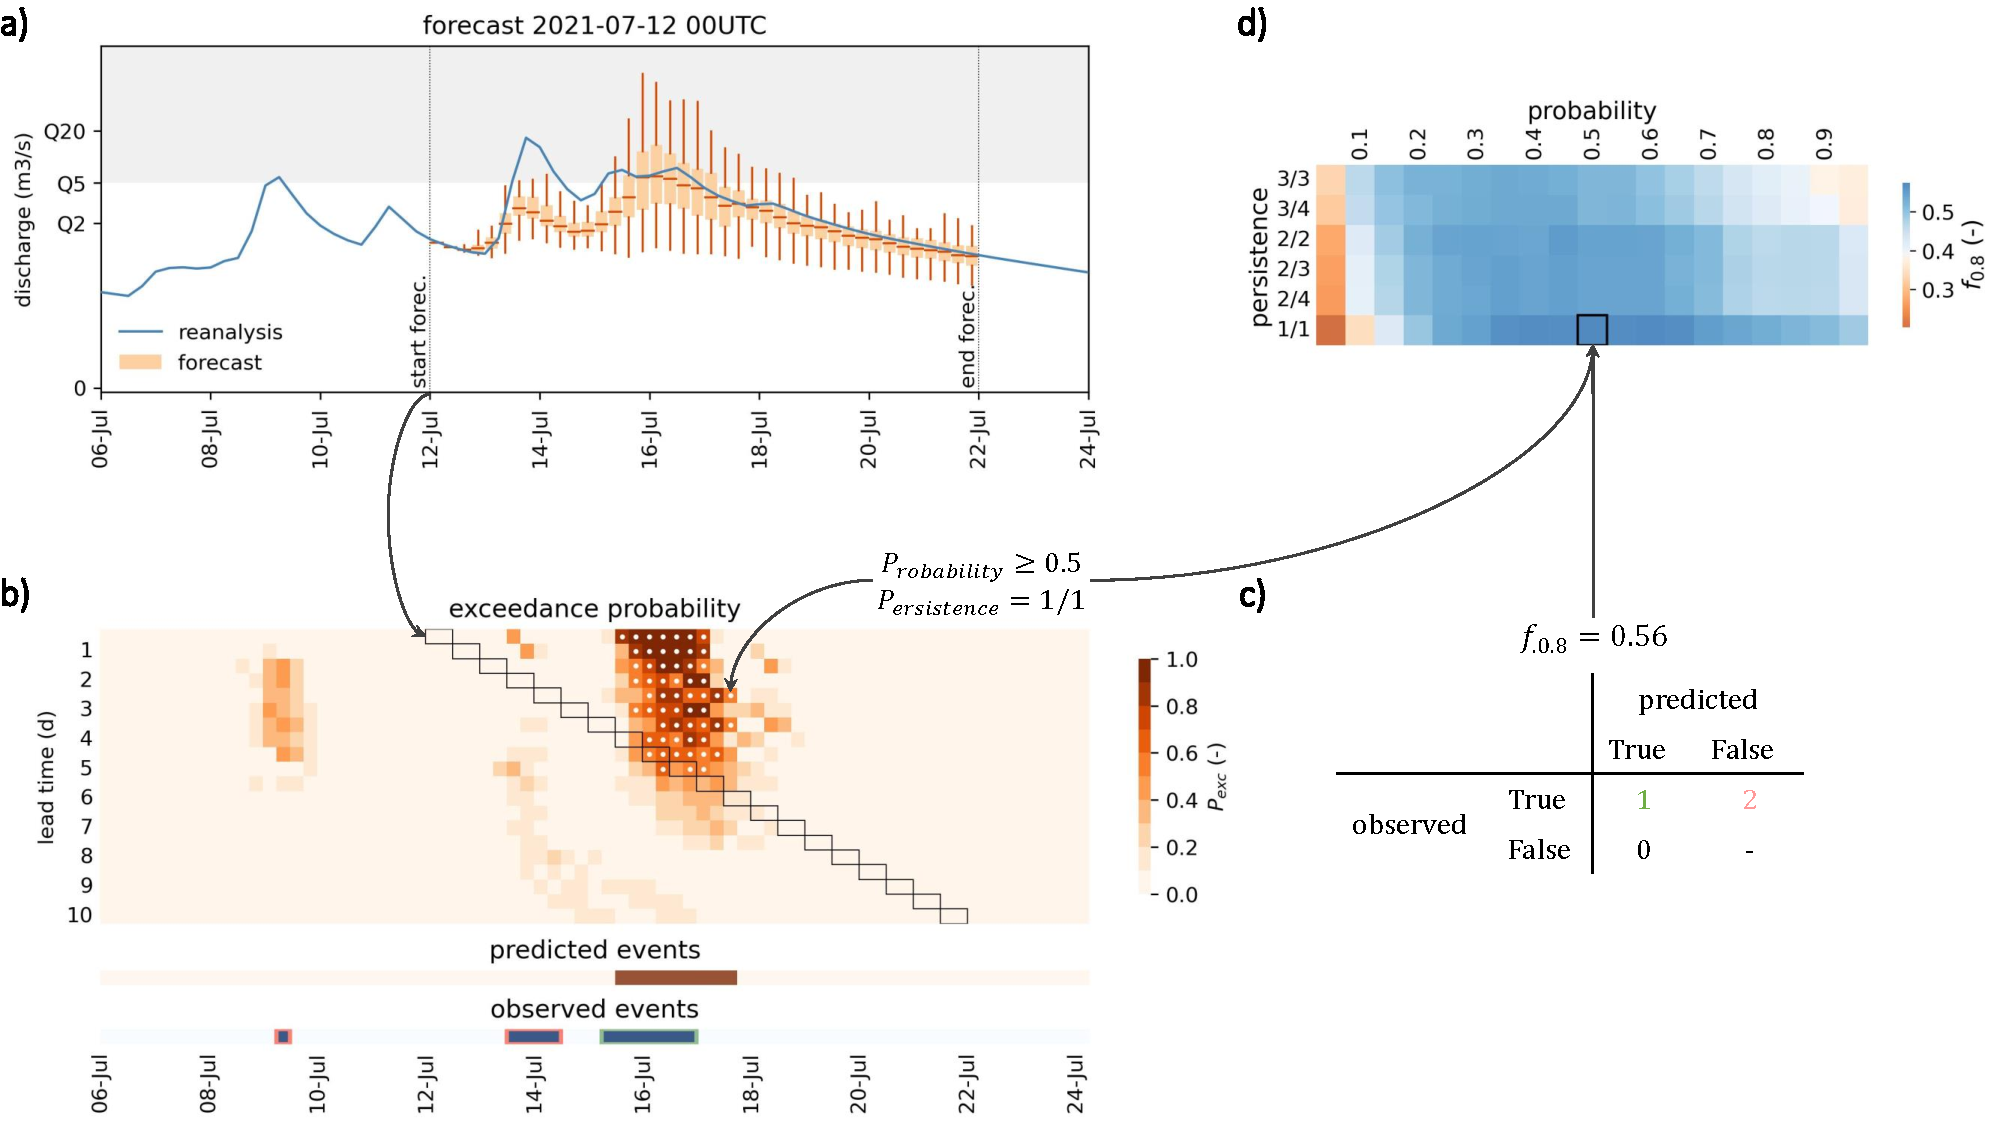
\includegraphics[width=1\textwidth]{figure01.pdf}
    \caption{Overview of the skill assessment framework. a) Hydrographs comparing observed and forecasted discharge with the discharge associated to the 5-year return period ($Q_5)$. b) Matrix of total exceedance probability —white dots identify cells that meet the warning criteria, whereas black rectangles delineate the location of the forecast hydrograph in panel (a)—, timeline of predicted events for that specific criteria, and timeline of observed events where hits are highlighted in green and misses in orange. c) Confusion matrix based on the previous warning criteria. d) Evaluation of the f-score across all combinations of probability threshold and persistence —the black square highlights the skill score corresponding to the warning criteria in panel (b)—.}
    \label{fig:scheme}
\end{figure*}

\subsection{Predicting flood events}
\label{sec:methods_prediction}

The warning process starts by converting the continuous time series of the target variable into time series of exceedance or non-exceedance over a predefined threshold. Since forecasts are issued more frequently  than the forecast horizon, they overlap. To address this, the ensemble forecasts are restructured into an exceedance probability matrix that connects each time step to increasing lead times, as illustrated in panel (b) of Figure \ref{fig:scheme}. Within this matrix, an individual forecast is represented by a diagonal (black rectangles). The uppermost rows represent shorter lead times, where the probability of accurate prediction generally increases. For instance, in the example in Figure \ref{fig:scheme}, the flood event occurring in July 16 was predicted with 50\% probability five days in advance, increasing close to certainty within two days of the event.

The derivation of the binary time series of observed events is straight forward by application of the  threshold over the discharge reanalysis. Conversely, deriving the binary time series of predicted events involves applying the warning criteria to the matrix of  probability of exceedance. The \textit{probability threshold} sets the minimum value of the exceedance probability at which a high risk of flooding is considered.  Additionally, the \textit{persistence} criterion removes false alarms caused by the erratic behaviour of some NWP \citep{Bartholmes2009}. This criterion aims to imitate the behaviour of a forecaster, who would wait to send the warning until consecutive forecasts predict the event. Panel (b) in Figure \ref{fig:scheme} illustrates the application of these two warning criteria on the matrix of exceedance probability. For every time step (columns in the total probability matrix), the white dots identify the lead times that meet the criteria. A flood event is predicted at a particular time step if any of the lead times meet the criteria.

\subsubsection*{EFAS current warning criteria}
\label{sec:methods_current_criteria}

Flood warnings in EFAS are based on discharge, and the critical threshold is the discharge associated with the 5-year return period ($Q_5$), computed by fitting a Gumbel distribution to the annual maxima in the EFASv4 long-term discharge simulation (1990-2022). While alternative alert systems might rely on disparate variables, such as precipitation \citep{Bouttier2024} or river stage \citep{Nevo2022}, and employ different thresholds for defining events, the underlying methodology remains similar. 

To issue a flood warning, five criteria must be met. EFAS warnings are exclusively issued to locations with a minimum catchment area of 2000 km² and for lead times longer than 48 hours. The first limit is based on the inferior hydrological performance in smaller catchments \citep{Alfieri2014}, while the second limit is a consequence of EFAS addressing early awareness and serving as a supplementary system to national or regional services. A warning is issued if at least one deterministic and one probabilistic NWP predict a probability of exceeding $Q_5$ larger than 30\% over 3 consecutive forecasts (hereafter referred to as 3/3 persistence). We denote this approach of combining the NWP models as  \textit{1 deterministic + 1 probabilistic} (1D+1P). As each model is evaluated independently, the current procedure does not calculate a total probability matrix. 

\subsection{Assessing warning skill}
\label{sec:methods_warning_skill}

\subsubsection{Contingency table}
\label{sec:methods_contingency_table}

Assessing the skill of a warning system is a binary classification task that compares two time series: the predicted and observed events. The contingency table (\ref{tab:contingency_table}) is commonly used to summarize the the performance of such tasks. Given that floods are rare events, the classification task is highly imbalanced, resulting in the number of true negatives being orders of magnitude larger than any of the other terms in the contingency table. Consequently, in order to avoid overestimating skill, we must omit the true negatives in the selection of the target skill metric (Section \ref{sec:methods_skill_metrics}). 

\begin{table}
    \centering
    \caption{Contingency table in a binary classification. $E_{obs}$ is the sum of observed events and $E_{pred}$ the sum of predicted events.}
    \begin{tabular}{ccccc}
        \toprule
        & & \multicolumn{2}{c}{Observed} & \\
        \cmidrule{3-4}
        & & True & False & \\
        \midrule
        Forecasted & True & hit & false alarm & $E_{pred}$ \\
        & False & miss & true negative & \\
        &  & $E_{obs}$ & & \\
        \bottomrule
    \end{tabular}
    \label{tab:contingency_table}
\end{table}

The terms of the contingency table result from comparing the time series of predicted and observed events. We consider a hit any observed event in which at least one time step was correctly predicted. The number of misses and false alarms are calculated as the difference between the observed ($E_{obs}$) or predicted ($E_{pred}$) events and the hits, respectively.

\begin{align}
    \label{eq:FN_FP}
    \text{misses} & = E_{obs} - \text{hits} \\
    \text{false alarms} & = E_{pred} - \text{hits}
\end{align}

The process is repeated for all possible combinations of the two criteria and across all stations. We tested probability threshold values ranging from 5\% to 95\% and six persistence values: 1/1 (no persistence), 2/4, 2/3, 2/2, 3/4 and 3/3.

\subsubsection{Skill metrics}
\label{sec:methods_skill_metrics}

The highly imbalanced nature of our classification tasks is fundamental in the selection of the skill metric. Metrics such as the odds ratio and the Hanssen-Kuipers score ($HK$) \citep{Hanssen1965}, which account for true negatives, are unsuitable for imbalanced classification and were thus excluded . Instead, we selected three metrics specific for imbalanced classification. 

Recall is the proportion of observed events that are correctly predicted (eq. \ref{eq:recall}). \citet{Bartholmes2009} proved that recall is equal to $HK$ for highly imbalanced classifications. Precision is the proportion of the predicted events that are correct (eq. \ref{eq:precision}). There is a well-known trade-off between recall and precision. Strict criteria result in fewer, more certain warnings, leading to high precision but low recall due to many missed events. Conversely, relaxed criteria increase the number of warnings, improving recall at the cost of precision due to a rise in false alarms. As a compromise, the $f_{\beta}$ score  is a metric that balances recall  and precision (eq. \ref{eq:fscore}). In its most common version ($\beta = 1$) it is the harmonic mean of recall and precision, granting equal importance to both terms. However, higher importance can be given to precision ($\beta < 1$), therefore limiting the amount of false alarms, or to recall ($\beta > 1$), reducing the number of misses. In our study, after suggestions from forecasters analysing EFAS on a daily basis, we selected $f_{0.8}$ as the target skill metric. This metric balances precision and recall giving a slightly higher value to the former. The idea behind is to limit the amount of false alarms, which would jeopardize the trust of the recipients of the warnings. Both recall, precision and the $f_\beta$ score range from 0 to 1, being 1 their optimal value.

As a final validation metric we used bias, which represents the proportion between the number of predicted and observed events  (eq. \ref{eq:bias}). Its optimal value is 1, which means that the number of warnings is equal to the number of observed events, and it ranges from 0 to infinity. All four metrics presented here can be plotted in the Roebber diagram \citep{Roebber2009} (Appendix C).

\begin{equation}
    \text{recall} = \frac{\text{hits}}{E_{obs}} = \frac{\text{hits}}{\text{hits} + \text{misses}}
    \label{eq:recall}
\end{equation}
\begin{equation}
    \text{precision} = \frac{\text{hits}}{E_{pred}} = \frac{\text{hits}}{\text{hits} + \text{false alarms}}
    \label{eq:precision}
\end{equation}
\begin{equation}
    f_{\beta} = \left( 1 + \beta^2 \right) \frac{\text{precision} \cdot \text{recall}}{\beta^2 \cdot \text{precision} + \text{recall}}
    \label{eq:fscore}
\end{equation}
\begin{equation}
    \text{bias} = \frac{E_{pred}}{E_{obs}} = \frac{\text{hits} + \text{false alarms}} {\text{hits} + \text{misses}} = \frac{\text{recall}}{\text{precision}}
    \label{eq:bias}
\end{equation}

\subsection{Combination of NWP}
\label{sec:methods_COMB}

One of the strengths of EFAS is the concurrent use of four NWPs, both deterministic and probabilistic. Using multiple NWPs serves two purposes: to allow national services to compare their forecasts with the corresponding EFAS simulations, and to leverage the strengths of different NWPs. In relation with this second purpose, a primary aim of this study is to develop an effective method for integrating deterministic and probabilistic forecasts. In practical terms, EFAS forecasts produce four distinct probability matrices, one for each NWP, in contrast to the single matrix depicted in panel (b) of Figure \ref{fig:scheme}. The challenge lies in devising a methodology to combine these four matrices into a total exceedance probability matrix, and enhance the system's predictive accuracy \citep{Wetterhall2013}. We explored three different approaches for calculating the total exceedance probability and compared them with the approach currently used in EFAS (Section \ref{sec:methods_current_criteria}).

The most straightforward method to compute the total probability is the \textit{model mean} (MM); it is a simple mean over the NWP-specific exceedance probability matrices, where all models are attributed equal weight. In this approach, the single member of a deterministic model is considered significantly more important than any individual member of a probabilistic model. An alternative approach would be to assign the same weight to each member. In this approach, referred to as \textit{member weighted} (MW), each NWP receives a weight relative to the number of members it contains, so probabilistic models prevail over deterministic ones. Neither of these approaches consider the performance of the NWP. To address this limitation, the \textit{Brier weighted} approach (BW) assigns a weight to each model based on its probabilistic skill. The Brier score  —a probabilistic error metric that ranges from 0 to infinite, with 0 being the optimal value— is used as a measure of probabilistic skill \citep{Brier1950}.

\begin{equation}
    \label{eq:BS}
    \text{BS} = \frac{1}{T}\sum_{t=1}^{T} \left( P_{obs,t} - P_{pred,t} \right)^2
\end{equation}

where $BS$  is the Brier score of a single station, $T$  is the number of time steps, $P_{obs,t}$ is the observed probability of exceedance, and $P_{pred,t}$  is the predicted probability of exceedance at a specific time step. We discovered that the results of the BW approach are highly sensitive to how Brier scores are converted into weights. The conversion function must invert $BS$ —as better models, with smaller $BS$, should receive higher weight—, and should be exponential to amplify the differences among NWP. Inverse distance weighing fulfils both conditions (eq. \ref{eq:IDW}). Values of the exponent $p$ from 1 to 9 were tested, and 7 was found to be the optimal exponent.

\begin{equation}
    \label{eq:IDW}
    w_{nwp,lt} = \frac{BS_{nwp,lt}^{-p}}{\sum_{i=1}^{4} BS_{i,lt}{-p}}
\end{equation}

\subsection{Optimising warning criteria}
\label{sec:methods_OPT}

Issuing a warning involves 5 criteria: minimum catchment area, minimum lead time, combination of NWP, probability threshold and persistence. We analysed each of these criteria individually to understand its effects, and then searched for the set of criteria that optimizes the system skill.

We have conducted two main experiments to explore the benefits of combining NWP. The first experiment analyses each NWP individually with two objectives: identifying the strengths and weaknesses of each NWP, and understanding how the warning criteria affect differently probabilistic and deterministic NWPs. The second experiment compares the four combinations of NWP explained in Section \ref{sec:methods_COMB}. The aim is to identify the most appropriate combination method and compare it against the most skilful NWP to assess whether the grand ensemble adds value to the system. The setup of these two experiments is similar and is explained in the following paragraphs.

For the majority of the analyses we used only stations that met the current minimum catchment area of 2000 km². With this subset of stations, we explored the evolution of skill with lead time, probability and persistence. Lead times were grouped in two ways. First, we grouped them daily to analyse the evolution of skill with lead time. Second, for the optimization of the warning criteria, we defined 4 lead time ranges: a) shorter than 2 days, a range at which EFAS warnings cannot be issued, b) 2-5.5 days, when all NWP are available, c) 5.5-7 days, when 3 NWP are available, d) 7-10 days, when only the ECMWF forecasts are available.

The optimization of the probability threshold and persistence criteria sought the combination of these two criteria that produces the maximum $f_{0.8}$ at each of the 4 lead time ranges. To ensure a robust selection of criteria, we applied a 10-fold cross validation: 20\% of the stations were left aside as a test set, while the remaining 80\% were subdivided in 10 folds. We computed the skill for every combination of 9 folds and then averaged over folds. The optimal warning criteria were derived from this average-over-fold skill matrix, as shown in panel (d) of Figure \ref{fig:scheme}. Subsequently, the selected criteria were evaluated on the test set to prevent overfitting. 

Lastly, we explored the impact of catchment area on warning skill using the entire set of stations. We calculated the warning skill for increasing values of the minimum catchment area, ranging from 500 km² to 300,000 km², using the previously optimized criteria.

\section{Results}
\label{sec:results}

\subsection{Analysis of individual NWPs}
\label{sec:results_NWP}

\subsubsection{Warning skill of individual NWPs}
\label{sec:NWP_skill}

Figure \ref{fig:NWP_skill_leadtime} exhibits the evolution of the warning skill with lead time and probability threshold for a scenario with no persistence.  As a benchmark, the skill of the current warning criteria is represented with a black, solid line. Each colour line represents a different probability threshold. For the two deterministic models (DWD and HRES) all lines overlap, since the probability threshold does not affect a deterministic forecast.

\begin{figure*}
    \centering
    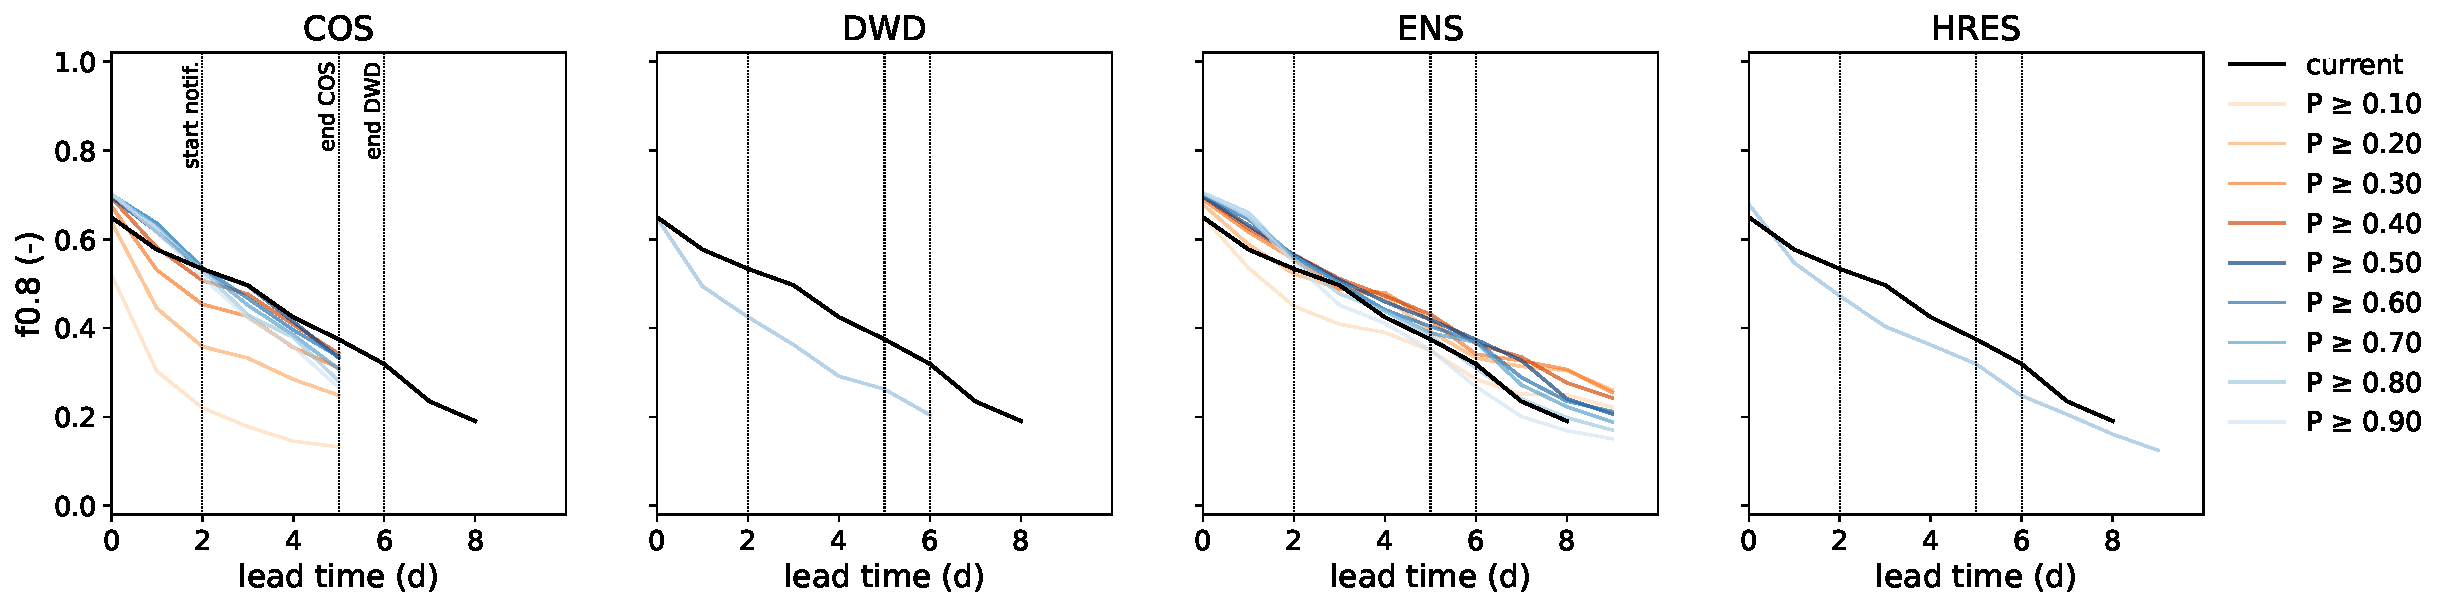
\includegraphics[width=1\textwidth]{figure02.pdf}
    \caption{Evolution of the warning skill with daily lead times and probability threshold for each NWP model in a scenario with no persistence. Each plot represents a different NWP. As a benchmark, the black, solid line represents the skill of the current operational criteria.}
    \label{fig:NWP_skill_leadtime}
\end{figure*}

The probabilistic models show overall higher skill than the deterministic. Under certain conditions, they even outperform the current warning criteria, indicating potential for enhancing the skill of EFAS. Deterministic models demonstrate skill on par with the current criteria solely for the first day forecast. As expected, warning skill degrades with lead time. This trend is consistent across all cases, although the rate of degradation depends on the probability threshold.

As we are seeking to identify a single optimal probability threshold for the warning criteria, the selection of the optimal criteria will prioritize a lead time range from 2 days to 5.5 days. This approach allows us to mitigate the substantial uncertainty associated with longer lead times, and focus on the lead times at which the majority of flood warnings are issued.

\subsubsection{Impacts of persistence on the warning skill of individual NWPs}
\label{sec:NWP_persistence}

Figure \ref{fig:NWP_skill_probability} illustrates the evolution of skill with probability threshold and persistence for a fixed lead time range (2-5.5 days). The benchmark (current warning criteria) is now represented by a single point. As the probability threshold does not affect deterministic forecasts, the lines for DWD and HRES are horizontal.

\begin{figure*}
    \centering
    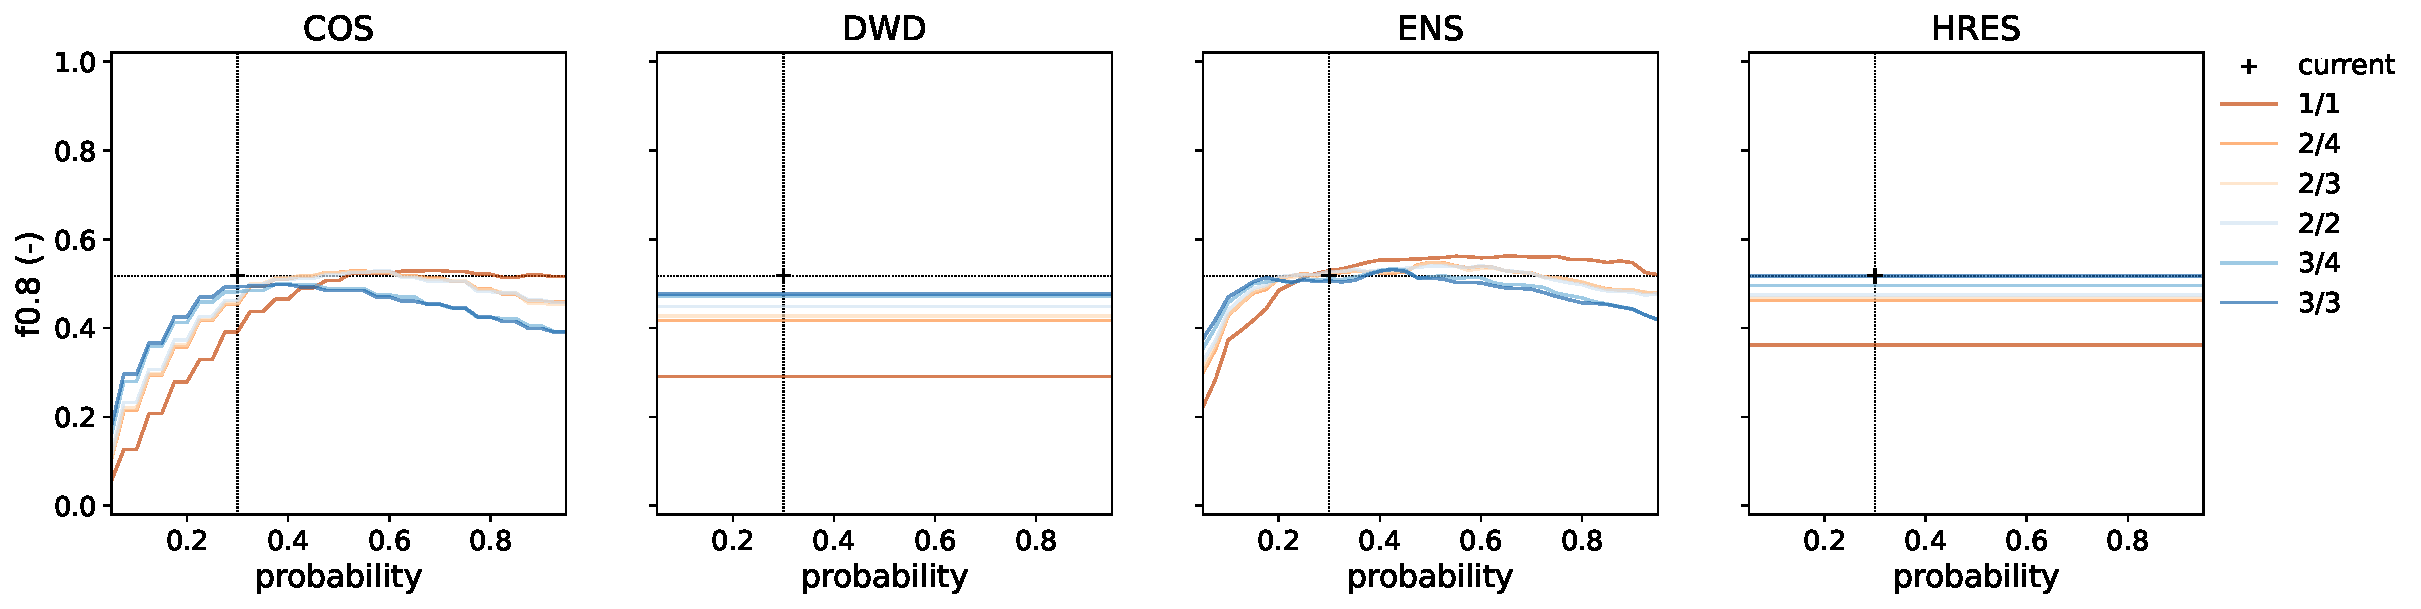
\includegraphics[width=1\textwidth]{figure03.pdf}
    \caption{Evolution of the warning skill with probability threshold and persistence  for each NWP model at a fixed lead time range (from 2 to 5.5 days). Each plot represents a different NWP model. As a benchmark, the black cross represents the current criteria.}
    \label{fig:NWP_skill_probability}
\end{figure*}

Three out of four NWPs are able to replicate or improve the skill of the current warning criteria at certain combinations of persistence and probability. Only DWD is less skilful than the benchmark. The skill of the probabilistic models shows a trade-off between probability threshold and persistence. Both criteria play the same role of removing false positives by taking stricter values. Consequently, stricter persistence necessitates lower probability thresholds to optimise skill, and vice versa. Nevertheless, the highest skill is consistently obtained when persistence is removed (1/1). In this scenario, there is a wide range of probability thresholds (from 40 to 90\%) that perform similarly well.

Persistence does have a significant impact in the skill of deterministic models, improving dramatically with the addition of any persistence. For the most stringent persistence (3/3), the skill of the deterministic HRES matches the benchmark.

\subsubsection{Optimal warning criteria for individual NWPs}
\label{sec:NWP_optimal_criteria}

The outcome of optimising the warning criteria for individual NWPs is summarised in Table \ref{tab:NWP_optimization}. The results are organised by lead time ranges; for each range, the table presents the optimized criteria and the skill metrics for the available NWPs. As a benchmark, the first row in each lead time range shows the skill of the current operational criteria. The Roebber diagram in Appendix C summarizes visually these results.
\begin{table*}
    \centering
    \caption{Summary of the optimization of the warning criteria for individual NWP and four lead time ranges. The initial row serves as a benchmark, indicating the skill of the current warning criteria. In each lead time range, bold fonts highlight the highest skill for a specific metric.}
    \begin{tabular}{cccccccc}
        \toprule
        lead time & model & probability & persistence & recall & precision & bias & $f_{0.8}$\\
        \midrule
        \textless 2 d & 1D+1P & 0.300& 3/3 & 0.522 & \textbf{0.735} & 0.710 & 0.634 \\
         & COS & 0.875 & 1/1 & 0.673 & 0.718 & 0.937 & \textbf{0.700} \\
         & DWD & - & 2/2 & 0.585 & 0.583 & \textbf{1.003} & 0.583 \\
         & ENS& 0.800 & 1/1 & \textbf{0.681} & 0.711 & 0.958 & 0.699 \\
         & HRES& -& 2/2 & 0.580 & 0.671 & 0.864 & 0.632 \\
         \midrule
        2-5.5 d & 1D+1P & 0.300& 3/3 & 0.413 & 0.618 & 0.668 & 0.518 \\
         & COS & 0.725 & 1/1 & 0.387 & 0.687 & 0.560 & 0.518 \\
         & DWD & - & 3/3 & \textbf{0.420} & 0.522 & \textbf{0.805} & 0.477 \\
         & ENS & 0.650 & 1/1 & 0.416 & \textbf{0.725} & 0.574 & \textbf{0.562} \\
         & HRES & - & 3/3 & 0.416 & 0.612 & 0.680 & 0.517 \\
         \midrule
        5.5-7 d & 1D+1P & 0.300& 3/3 & 0.215 & \textbf{0.612} & 0.351 & 0.356 \\
         & DWD & - & 2/2 & \textbf{0.291} & 0.358 & \textbf{0.813} & 0.328 \\
         & ENS & 0.450 & 1/1 & 0.264 & 0.605 & 0.436 & \textbf{0.402} \\
         & HRES & - & 2/2 & 0.273 & 0.429 & 0.636 & 0.351 \\
         \midrule
        7-10 d & 1D+1P & 0.300& 3/3 & 0.120 & \textbf{0.625} & 0.192 & 0.237 \\
         & ENS & 0.175 & 2/2 & \textbf{0.287} & 0.396 & 0.725 & \textbf{0.345} \\
         & HRES & - & 2/2 & 0.244 & 0.336 & \textbf{0.726} & 0.293 \\
         \bottomrule
    \end{tabular}
    \label{tab:NWP_optimization}
\end{table*}

The current EFAS setup (1D+1P) is negatively bias, i.e., prioritizes precision over recall. Warnings are issued with a high level of certainty, leading to a limited number of false alarms, but many events are missed. The current criteria are not optimal as it is consistently outperformed in terms of $f_{0.8}$ at any lead time by individual NWPs, suggesting that the current combination of all NWPs hinders the skill of that single best NWP.

The analysis of the results is similar for any of the four lead time ranges. The probabilistic NWPs (COS and ENS) constantly outperform in terms of $f_{0.8}$ both the benchmark and the deterministic counterparts. Even though both probabilistic NWPs show similar skill at the shortest lead time, ENS stands out as the best model at medium-range forecasts. The skill of HRES, despite being deterministic, is comparable to the benchmark, even outperforms it at the longest lead time. Overall, the optimization of individual NWPs was able to increase the warning skill by up to 6.6\%.

The optimization removed the persistence criterion for the probabilistic NWPs. Its role  —removing uncertain events— is now played solely by the probability threshold. The optimal value of this probability threshold is very high at short lead times and decreases with increasing lead time, being larger than the current value up to lead time 7 days. On the contrary, deterministic models require persistence to enhance their skill, although there is not a clear pattern between the optimal persistence and lead time.

\subsection{Analysis of combined NWPs}
\label{sec:results_COMB}

\subsubsection{Weighing matrices}
\label{sec:weights}

Three of the four combination methods compute total probability, which requires assigning weights to each NWP and lead time. Figure \ref{fig:weights} illustrates the distribution of weights among NWP models for these three combination methods.

\begin{figure*}
    \centering
    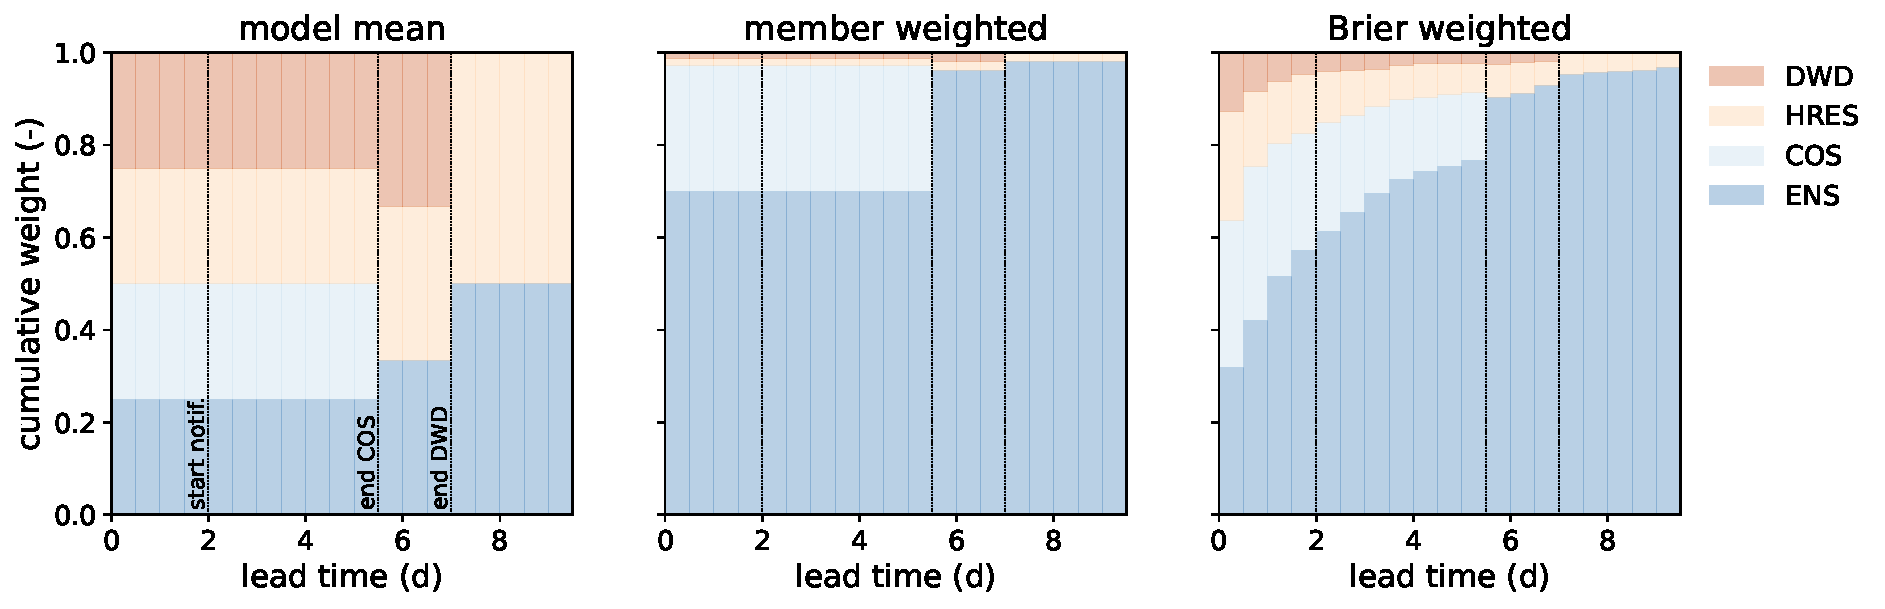
\includegraphics[width=0.8\textwidth]{figure04.pdf}
    \caption{Weights applied to compute total probability. Every plot represents a different method, with colours representing NWPs (blue for probabilistic and orange for deterministic models).}
    \label{fig:weights}
\end{figure*}

The \textit{model mean} (MM) attributes equal weights to each model. The changes in the weight distribution occur when the maximum lead time of a model is exceeded. This  approach assigns equal importance to deterministic and probabilistic models.

Instead, in the \textit{member weighted} (MW) combination, every model run is assigned an equal weight. ENS, which has a significant larger number of members, prevails over any other NWP. Even for the first 5 days, when all the models are available, ENS receives 70\% of the weight. In general, this approach heavily relies on the skill of the largest ensemble, which is not necessarily the most skilful.

In the \textit{Brier weighted} (BW) combination, we used the Brier score (\ref{appendix:NWP_prob_skill}) to derive weighing factors that prioritize the more skilled models. At very short lead times, the deterministic models demonstrate skill (Figure \ref{fig:BSS}), accounting for approximately a third of the total weight. As the lead time increases, the probabilistic models, particularly ENS, assume the majority of the weight. At lead times from 2 to 5.5 days, when most of the warnings are sent, the superior skill of probabilistic models is represented by a combined weight of approximately 80\%.

\subsubsection{Warning skill of combined NWPs}
\label{sec:COMB_skill}

Figure \ref{fig:COMB_skill_leadtime} replicates the analysis of the warning skill previously done for the individual NWP models, but for the combination methods. It exhibits the evolution of the warning skill with lead time and probability threshold for a an scenario without persistence. The benchmark is ENS, the NWP that proved highest skill.

\begin{figure*}[ht]
    \centering
    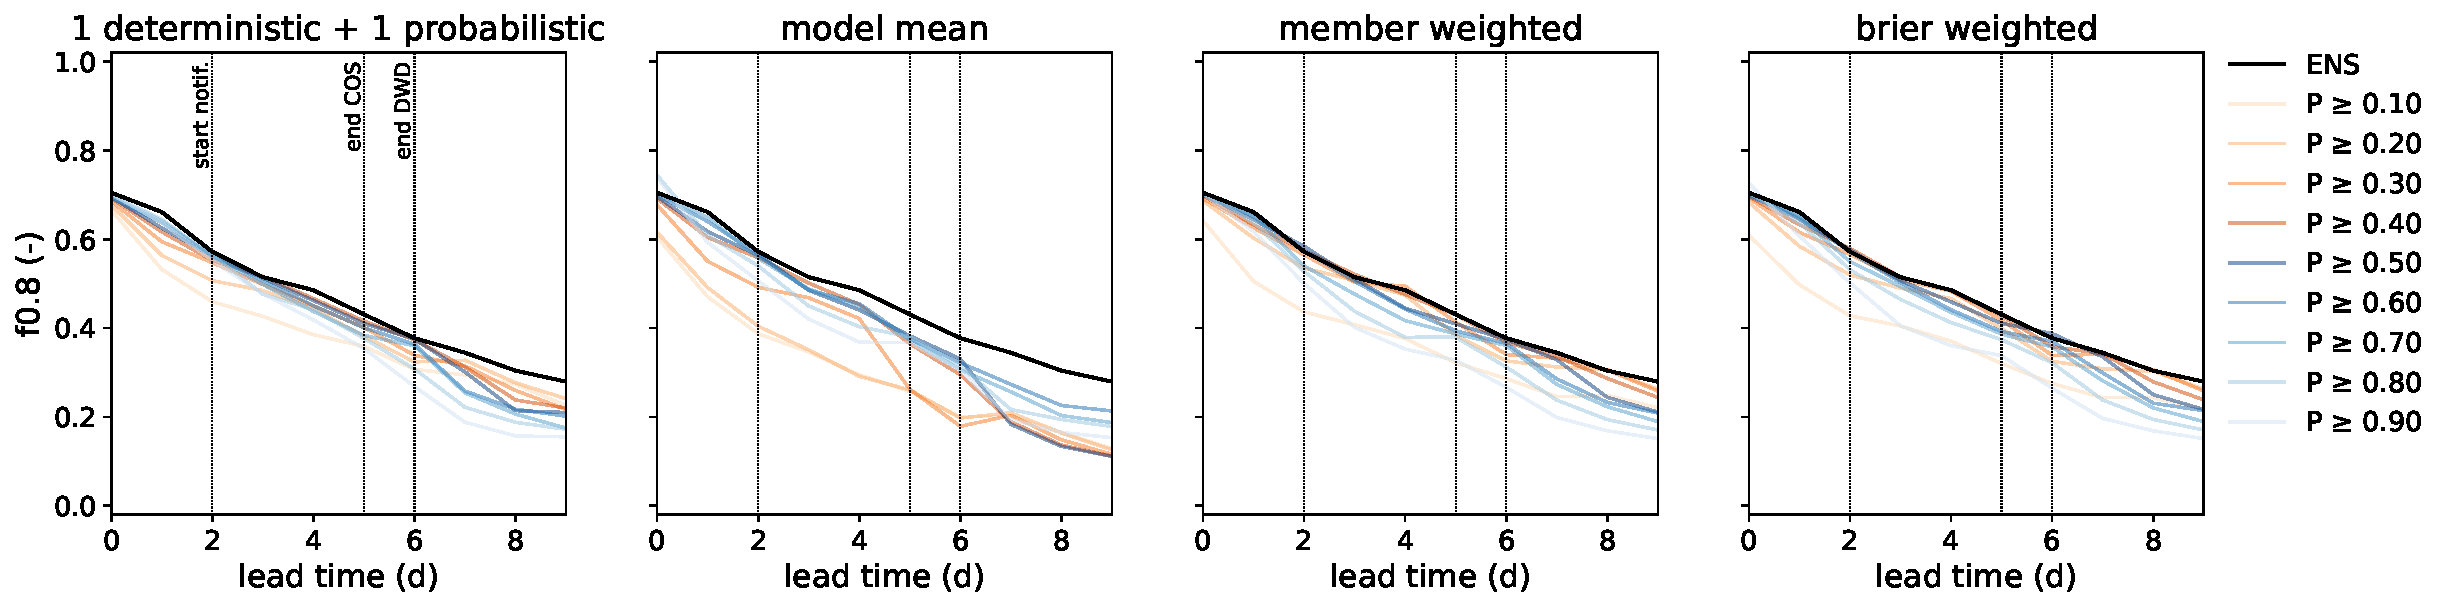
\includegraphics[width=1\textwidth]{figure05.pdf}
    \caption{Evolution of the warning skill at daily lead times and probability threshold for each of the combination methods in a scenario with no persistence. Each plot represents a different combination of NWP. As a benchmark, the black, solid line represents the skill of ENS with optimised criteria.}
    \label{fig:COMB_skill_leadtime}
\end{figure*}

The results indicate that ENS is responsible for the majority of the skill in the grand ensembles, since only marginal gains are possible with specific combinations at certain lead times. Only two combination methods (MW and BW) are able to replicate the skill of the benchmark across all lead times. Although MM at lead time 0 achieves the highest marginal gain, this combination method is not suitable as its skill is poorer than the benchmark from day 2 onwards. The current procedure (1D+1P) is also sub-optimal, even though the degradation with lead time is not as severe as in MM.

\subsubsection{Impacts of persistence on the warning skill of combined NWPs}
\label{sec:COMB_persistence}

Figure \ref{fig:COMB_skill_probability} presents the evolution of the gran ensemble skill with probability and persistence for a fixed lead time range (2-5.5 days). The black cross represents the skill of ENS with its optimal warning criteria.

\begin{figure*}
    \centering
    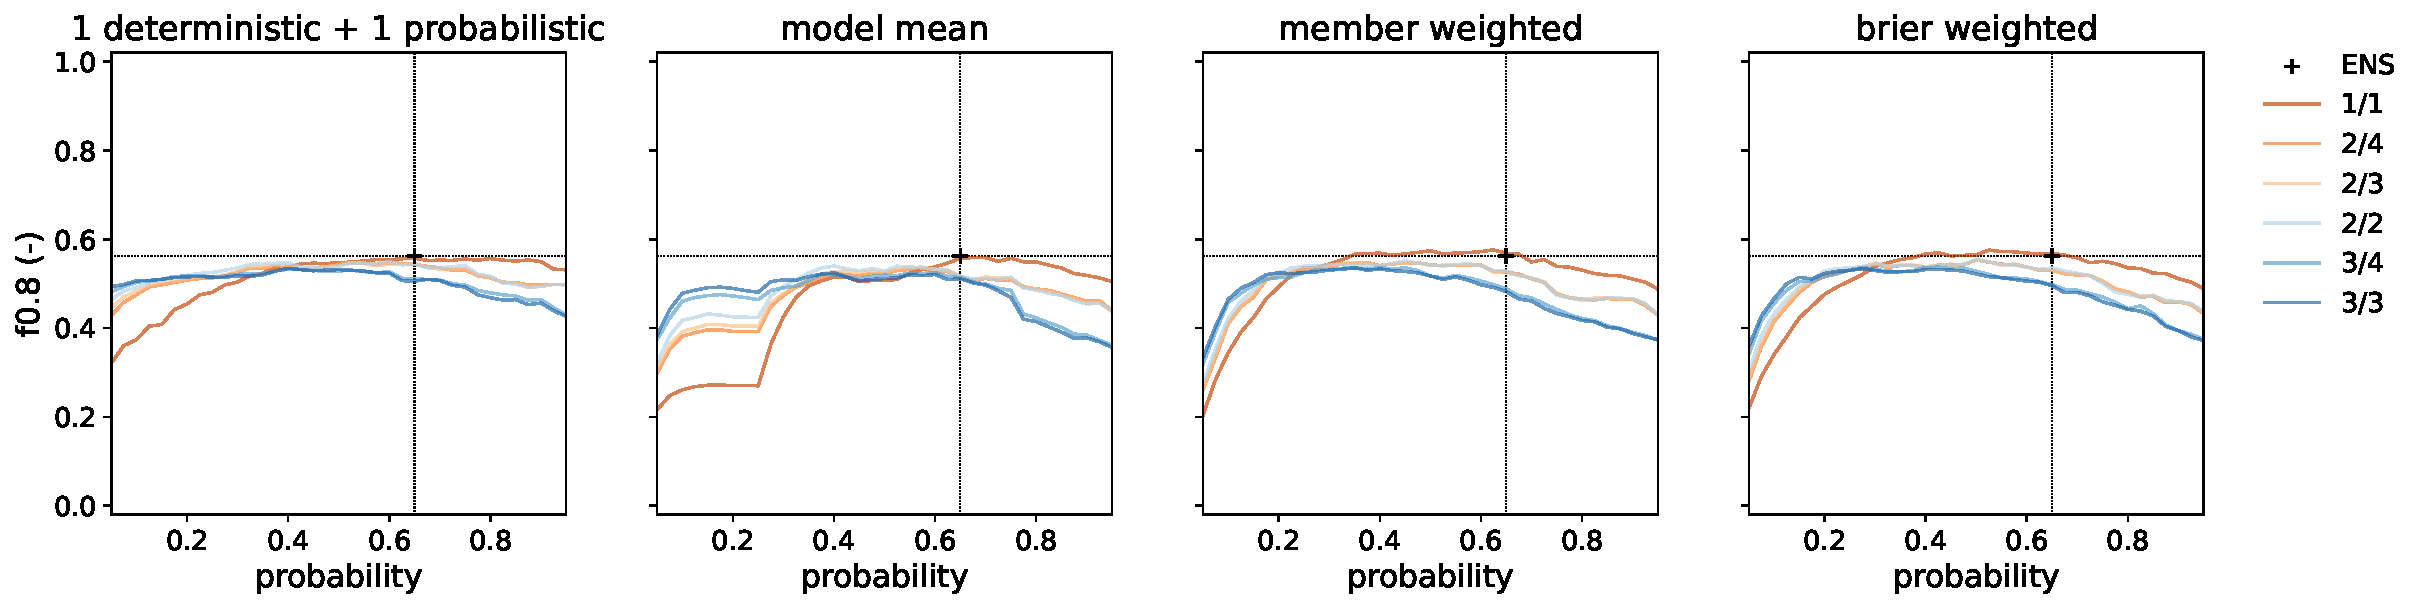
\includegraphics[width=1\textwidth]{figure06.pdf}
    \caption{Evolution of the warning skill with probability threshold and persistence  for each combination of NWP at a fixed lead time range (from 2 to 5.5 days). Each plot represents a different combination of NWP. As a benchmark, the black cross represents the skill of ENS with optimised criteria.}
    \label{fig:COMB_skill_probability}
\end{figure*}

The results reinforce the idea that the persistence criterion limits the maximum attainable skill in ensemble systems. Across all four combinations, the highest skill is reached when persistence is removed (1/1). In this scenario, all combinations exhibit similar maximum skill. Only member weighted (MW) and Brier weighted  (BW) marginally surpass the benchmark (ENS). These two combinations show optimal skill within a range of probability thresholds spanning 40\% to 70\%.

The lack of sensitivity to probability is notable in the current criteria, indicated by the dark blue line in the left-hand side pane. Even at the lowest probability threshold, the $f_{0.8}$ score remains at 0.5, unlike other combinations that exhibit a significant decline in performance when the probability threshold takes very low values.

\subsubsection{Optimal warning criteria for combined NWPs}
\label{sec:COMB_optimal_criteria}

Table \ref{tab:COMB_optimization} summarizes the results of the optimization of the warning criteria for the combination methods in an identical way as Table \ref{tab:NWP_optimization} did for the NWP. The results are organised by lead time ranges; for each range, the table presents the optimized criteria and the skill metrics for the four methods. As a benchmark, the first row in each lead time range shows the skill of ENS. A graphical summary of these results can be seen in Appendix C.
\begin{table*}[ht]
    \centering
    \caption{Summary of the optimization of the warning criteria for the combination methods and four lead time ranges. The initial row serves as a benchmark, indicating the skill of ENS, the top-performing NWP. In each lead time range, bold fonts highlight the highest skill for a specific metric. }
    \begin{tabular}{cccccccc}
        \toprule
        lead time & method & probability & persistence & recall & precision & bias & $f_{0.8}$ \\
        \midrule
        \textless 2 d& ENS & 0.800 & 1/1 & \textbf{0.681} & 0.711 & \textbf{0.958} & 0.699 \\
         & 1D+1P & 0.925 & 1/1 & 0.662 & 0.717 & 0.923 & 0.694 \\
         & MM & 0.775 & 1/1 & 0.628 & \textbf{0.838} & 0.749 & \textbf{0.741} \\
         & MW & 0.750 & 1/1 & 0.673 & 0.718 & 0.937 & 0.700 \\
         & BW & 0.950 & 1/1 & 0.620 & 0.829 & 0.748 & 0.733 \\
         \midrule
        2-5.5 d & ENS & 0.650 & 1/1 & 0.416 & \textbf{0.725} & 0.574 & 0.562 \\
         & 1D+1P & 0.600 & 1/1 & \textbf{0.455} & 0.643 & \textbf{0.708} & 0.554 \\
         & MM & 0.700 & 1/1 & 0.424 & 0.700 & 0.606 & 0.559 \\
         & MW & 0.500 & 1/1 & \textbf{0.455} & 0.692 & 0.658 & 0.574 \\
         & BW & 0.525 & 1/1 & 0.451 & 0.700 & 0.644 & \textbf{0.576} \\
         \midrule
        5.5-7 d & ENS & 0.450 & 1/1 & 0.264 & \textbf{0.605} & 0.436 & \textbf{0.402} \\
         & 1D+1P & 0.425 & 1/1 & 0.262 & 0.599 & 0.437 & 0.399 \\
         & MM & 0.500 & 1/1 & \textbf{0.276} & 0.412 & \textbf{0.670} & 0.345 \\
         & MW & 0.425 & 1/1 & 0.271 & 0.579 & 0.468 & 0.401 \\
         & BW & 0.450 & 1/1 & 0.268 & 0.586 & 0.457 & 0.400 \\
         \midrule
        7-10 d & ENS & 0.175 & 2/2 & \textbf{0.287} & 0.396 & 0.725 & \textbf{0.345} \\
         & 1D+1P & 0.250 & 1/1 & 0.256 & 0.414 & 0.618 & 0.334 \\
         & MM & 0.225 & 2/2 & 0.252 & 0.334 & \textbf{0.754} & 0.296 \\
         & MW & 0.175 & 2/2 & 0.278 & 0.402 & 0.692 & 0.343 \\
         & BW & 0.300 & 1/1 & 0.255 & \textbf{0.445} & 0.573 & \textbf{0.345} \\
         \bottomrule
    \end{tabular}
    \label{tab:COMB_optimization}
\end{table*}

The benchmark (ENS) is only outperformed in terms of $f_{0.8}$ by some combinations at lead times shorter than 5.5 days. At the shortest lead time range, the inclusion of deterministic NWPs is important as they have notable skill (see Figure \ref{fig:BSS}). For this reason, the two combination methods that allocate higher weight to deterministic models (MM and BW) show the highest skill. At lead times from 2 to 5.5 days, BW and MW stand out as the best approaches. They prove comparable skill and optimize similar criteria due to the fact that they give a similar weight to ENS, as it is both the NWP with the largest number of members and with the highest skill. It is worth noting that the combination currently used in EFAS (1D+1P) is the only approach that never outperforms the benchmark. Overall, the optimal grand ensemble can achieve an improvement in skill up to 4.2\% compared with ENS (up to 10\% compared with the current criteria).

The optimised criteria show a pattern similar to that observed in the individual NWPs. The persistence criterion is removed in all the combinations at lead times shorter than 7 days. The probability threshold replaces the role of persistence, adopting optimal values notably larger than in the current criteria that decrease with increasing lead time.

\subsubsection{Optimal versus current warning skill}
\label{sec:COMB_vs_current}

The maps in Figure \ref{fig:maps_BW} illustrate the skill metrics associated with the best grand ensemble —BW  with no persistence and a probability threshold of 52.5\%— for the lead time range 2 to 5.5 days.
\begin{figure*}[ht]
    \centering
    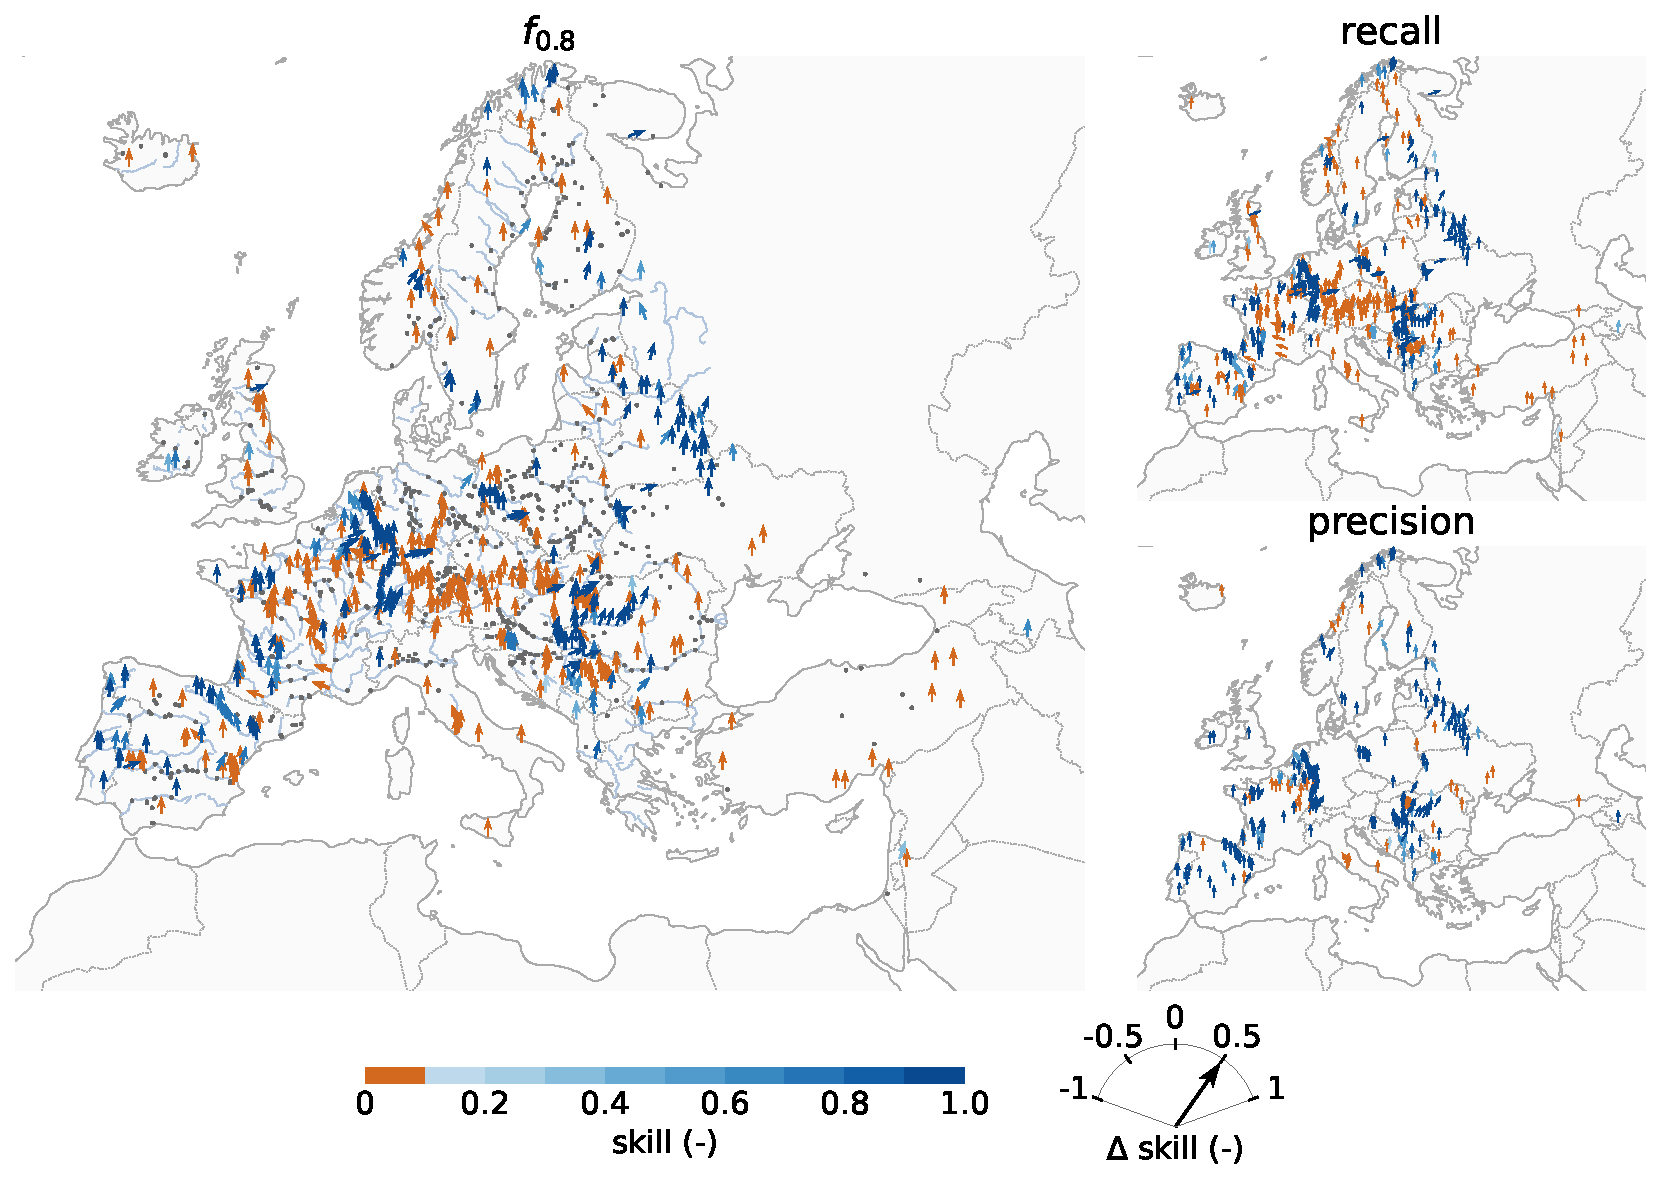
\includegraphics[width=1\linewidth]{figure07.pdf}
    \caption{Skill maps for the optimised warning criteria (BW, 52.5\% probability  and no persistence) at the lead time range from 2 to 5.5 days. The main plot shows the skill in terms of $f_{0.8}$; grey dots are stations for which the f-score cannot be computed due to all instances of hits, misses and false alarms being null. The smaller plots show precision and recall; for the sake of visibility, it only shows the stations for which the specific metric can be computed. In all the plots the direction of the arrows shows the difference in skill between the optimised and the current criteria; positive values imply gains and negative values losses in skill.}
    \label{fig:maps_BW}
\end{figure*}

A pronounced contrast is evident in the maps, attributable to the limited number of events in most of the stations, resulting in skill metrics primarily yielding values of either 1 or 0. In terms of $f_{0.8}$, there is a cluster of underperforming points in central Europe (notably the Alps) and central France. The decomposition into recall and precision reveals that the primary contributor to the low f-score is recall, indicating missed events. Conversely, the precision of warnings remains consistently high, with exceptions observed in the Seine and Arno rivers. It is noteworthy the skill in all metrics for the Ebro, Rhine and Meuse—three rivers that experienced significant flood events during the study period.

By applying the optimised criteria, EFAS would be able to predict with at least 2 days lead time 46\% of the events, and 71\% of all the warnings would be correct. For reference, these figures represent an improvement in both metrics over the existing criteria, which achieved 41\% recall and 62\% precision.

\subsubsection{Influence of catchment area on warning skill}
\label{sec:skill_area}

The preceding sections presented results for a set of stations with a catchment area of at least 2000 km², the current limit in EFAS. To investigate the potential relaxation of this criterion, Figure \ref{fig:skill_area} illustrates the evolution of skill depending on the catchment area limit. The criteria used to create this figure are those optimized for the fixed area limit of 2000 km² and a lead time range from 2 to 5.5 days (Table \ref{tab:COMB_optimization}). The plot compares the skill of the four combination methods (coloured lines) with the skill of the current warning criteria (black line).

\begin{figure*}
    \centering
    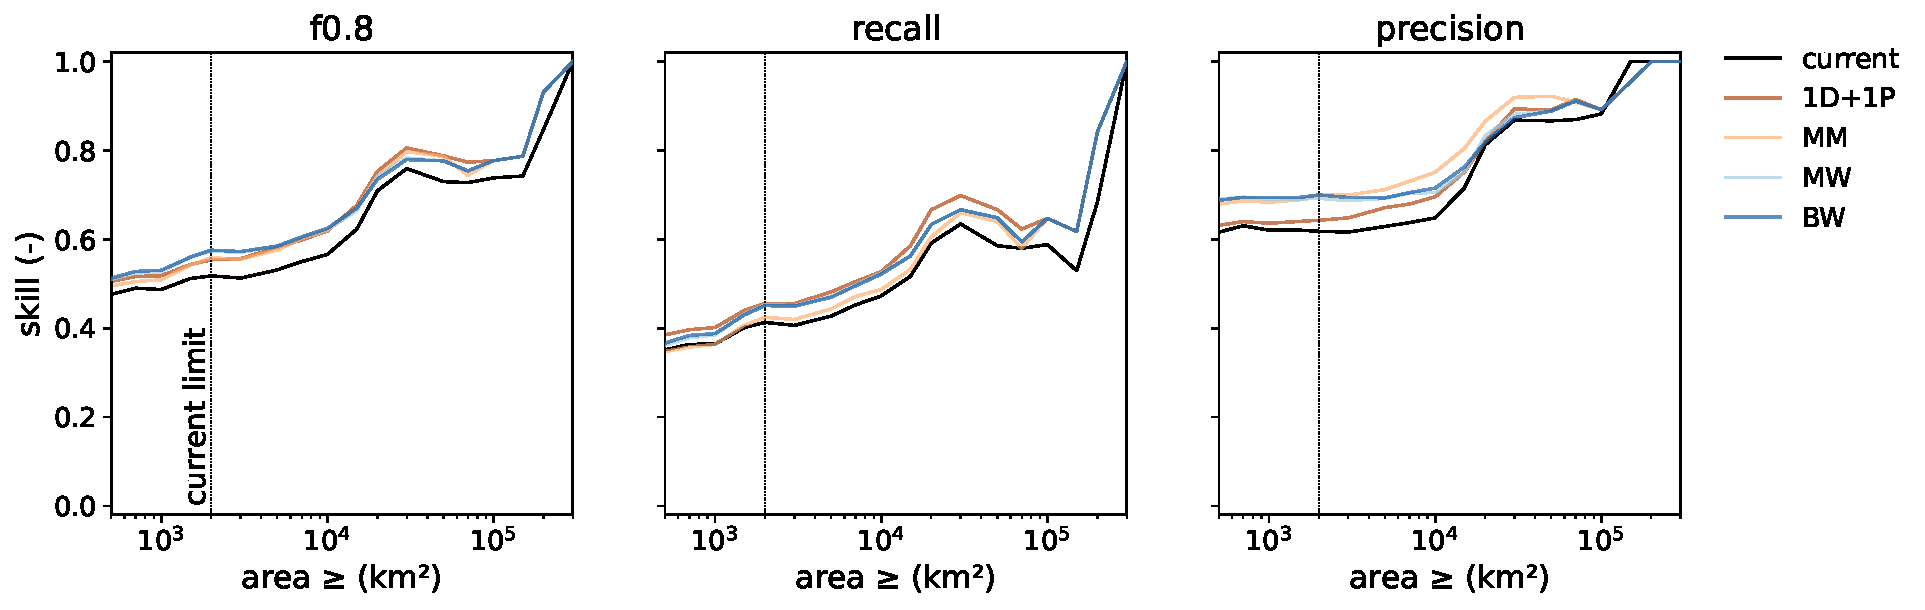
\includegraphics[width=0.8\linewidth]{figure08.pdf}
    \caption{Evolution of skill with catchment area limit. Each plot represents a skill metric. In each of the plots, the black line represents the skill of the current warning criteria, while the colour lines depict the skill of the optimized criteria for the 4 combination methods. The vertical, dotted line indicates the catchment area limit currently applied in EFAS.}
    \label{fig:skill_area}
\end{figure*}

The skill of the system improves with catchment area, as expected. However, the skill curves do not increase continuously. Recall experiences a loss in skill for areas ranging from 30,000 to 70,000 km², leading to a decrease in $f_{0.8}$. This loss is caused by missed events in the Guadiana, Seine, Loire, Rhone and Danube catchments. As already mentioned in previous sections, there is a notable gap between recall and precision in both the optimised and current warning criteria, with precision consistently surpassing recall. 

The vertical line at 2000 km² illustrates the gain in skill achieved with the optimization, which is sustained across all catchment area values. Reducing the catchment area limit results in minimal loss in $f_{0.8}$, suggesting that this criterion could be relaxed without compromising skill. For instance, the BW combination at 1,000 km²  exhibits slightly higher skill ($f_{0.8}=0.531$) than the current criteria at 2000 km² ($f_{0.8}=0.518$). The relaxation of the catchment area limit impacts the components of the f-score differently. While precision remains unaffected, there is a loss in recall.

\section{Discussion}
\label{sec:discussion}

\subsection{Limitations and moving forward}
\label{disc:limitations}

The definition of the spatial and temporal framework is often a limitation in studies that assess the skill of ensemble flood forecasting systems \citep{Pappenberger2008a, Cloke2009}. Due to the rarity of flood events, the statistical robustness of such analysis relies on a limited and often highly correlated sample of events. To address this limitation, long-term and continental or global studies are advocated, such as the one presented here, which spans over a period of two and a half years and extends over a European domain. Nevertheless, our study would benefit from a larger sample of points and flood events. As shown in Figure \ref{fig:maps_BW}, there are many stations for which the skill metrics cannot be calculated due to null hits, misses or false alarms. A larger sample of observed events would reduce the susceptibility of the analysis to this issue. Two potential solutions emerge: extending the study period, which is limited by the availability of the HEPS forecasts, or using an event threshold of higher recurrence. We decided to work with a sample of stations, instead of all the river cells \citep{Bartholmes2009}, to limit the spatial correlation of events.

In the optimization of the warning criteria, we set a catchment area limit of 2,000 km², a threshold inherited from previous EFAS setups with lower spatial and temporal resolution. The results of this study  demonstrate that the current resolution of both NWP and hydrological models can produce comparably skilful warnings at smaller catchments (Figure \ref{fig:skill_area}), which can significantly increase the number of stations and flood events analysed (\ref{fig:observed_vs_area}). In line with this, the new EFASv5 \citep{EFASv5.0} released in September 2023 increased spatial resolution from 5 km to 1 arc-minute, which is expected to further improve the skill of the system in smaller catchments. The skill of this new EFAS version will be analysed as soon as a long enough period or reforecasts are available.

The selection of the target metric is a critical aspect in any skill analysis. \citet{Bartholmes2009} reviewed the desired characteristics of a skill score, and selected odds ratio, $HK$ score and bias as their target metrics. In contrast, we selected the $f_{\beta}$ score, a metric commonly used in machine learning, but rarely applied in hydrology. The $f_{\beta}$ score has two interesting properties for analysing a flood warning system. Firstly, it is based on the contingency table but avoids using true negatives, which could overestimate skill. Secondly, it allows for tailoring the warning criteria to the specific use case, as the $\beta$ parameter can be adjusted to penalize differently misses or false alarms. For instance, \citet{Bouttier2024} used the $f_2$ score to optimize the probability threshold for high-intensity precipitation warnings in France. The $\beta$ value of 2 penalizes four times more missed events than false alarms, under the assumption that the cost of  being hit by an extreme event unprepared is larger than the cost of mobilising resources in a false alarm. In our study, we took the opposite approach and decided to minimize the number of false alarms by using a $\beta$ value of $0.8$. This decision was based on the fact that EFAS complements the national or regional systems by issuing medium-range flood warnings. The aim is to alert authorities, not the general public, only when there is substantial evidence that the event will occur, in order to avoid excessive warnings that could undermine their trust in the system. Additionally, the event threshold (5-year return period) corresponds to a recurrence time shorter than the flood protection levels in many European regions, so we assume that missing minor events will not be as costly as \citet{Bouttier2024} argue. In a preliminary analysis, we tested $\beta$ values of 0.8, 1 and 1.25 and found that the changes in the f-score were minimal (in the order of 3\%) and in none of the cases persistence was needed. However, the selection of $\beta$ affects the optimal probability threshold and the resulting bias, i.e., the distribution of errors between misses and false alarms. Such decision should be taken in collaboration with the end users to tailor the warnings to their specific needs \citep{Lavers2020, Dasgupta2023}.

\subsection{Addressing study objectives}
\label{disc:objectives}

The first objective of this study was to evaluate the skill of the different NWPs within EFAS, with a specific focus on comparing deterministic and probabilistic models. Figure \ref{fig:BSS} demonstrates that probabilistic NWPs outperform deterministic models in terms of Brier skill score across all lead times. Only at short lead times do deterministic NWPs reach similar levels of skill. The outcome is similar when applying the warning criteria and measuring warning skill in terms of $f_{0.8}$ (Table \ref{tab:NWP_optimization}). At their optimal warning criteria, the probabilistic NWPs, particularly ENS, outperform deterministic NWPs. The skill of both types of NWP degrades with increasing lead time, casting doubt on their ability to issue flood alerts more than 7 days in advance. The effects of the probability threshold and persistence criteria differs depending on the nature of the NWP. The probability threshold has a substantial effect on the skill of probabilistic models, while it does not impact deterministic models. Both COS and ENS perform better at probability thresholds over 50\%, with a wide range of similarly performing values. On the contrary, persistence proves to be beneficial in improving the warning skill of deterministic NWPs, but it limits the skill of probabilistic models. Persistence, a.k.a. poor man's ensemble, is a method of creating an ensemble out of a deterministic forecast \citep{Cloke2009}. For instance, a persistence of 3/3 is an ensemble of 3 members with a probability threshold of 100\%. Our results show that while persistence removes the inherent erratic behaviour of deterministic models and notably improves their skill, it should not be applied to HEPS. 

The second objective of this study was to determine the appropriate method to combine several NWP models into a grand ensemble. Careful consideration is necessary in selecting this method to avoid diminishing the skill of the most proficient NWP within the grand ensemble. For instance, the current EFAS warning criteria limit the skill of the system to that of the highest-performing deterministic model (HRES). This limitation is caused by a combination method that excessively relies on deterministic forecasts, as well as the use of persistence. The challenge lies in finding a combination that enhances the skill of the best-performing NWP, which in the case of EFAS is ENS.

Our findings demonstrate that ENS is a very strong baseline, with only a few combination methods yielding gains to its skill. These findings contrast slightly with \citet{Pappenberger2008b}, who showed for a specific flood event in Romania in 2007 that grand ensembles can detect extreme events that a single EPS could entirely miss. In our study case, the effectiveness of the grand ensemble is limited to the first 5 days lead time. Overall, the most promising approaches are the member-based (MW) and skill-based (BW) methods. Both methods have similar optimal warning criteria (no persistence and a probability threshold close to 50\%), and their success is based on granting most of the weight to ENS. However, the reason why they allocate this weight to ENS differs. In the case of MW, it is coincidental that the most skilful model also possesses the largest number of members. On the contrary, BW grants greater value to ENS because it proved to be a superior model. If a more skilful model with fewer members would be added to the grand ensemble, BW would be able to extract that skill, while MW would not. Therefore, we argue that skill-based combination methods are preferable. 

\subsection{Towards operationalization}
\label{disc:operationalization}

The decision on the most appropriate combination method cannot be based solely on skill metrics, but also consider other factors such as the  operational implementation effort, user comprehensibility, or the impact of adding or removing a NWP. Skill-based approaches, such as BW, are theoretically superior as they allocate weights based on quality rather than quantity. They are also the most robust when it comes to adding or removing NWPs. However, they are more challenging to implement and to explain to end users. To derive the matrix of weights (Figure \ref{fig:weights}), a skill-based approach requires an extensive period of reanalysis and reforecasts upfront, posing a substantial computational burden on system implementation. Additionally,  practitioners using the forecasts would require additional training to understand that the ensemble members are not equiprobable, which would be more intuitive.

There remains a question on the use of deterministic models in a grand ensemble dominated by a probabilistic NWP. When using a member-based combination, such as MW, deterministic models could be removed from the grand ensemble, as the weight allocated to them is so small that their inclusion barely affects the total probability. Skill-based approaches, instead, allocate larger weights to these models in the very first lead times, when they have proven skill given their often-higher resolution. The inclusion of deterministic models is a topic for future analysis, as the spatial resolution of deterministic and probabilistic NWP are nowadays similar, and centres such as ECMWF plan to discontinue their deterministic models in favour of the ensembles.

\section{Conclusions}
\label{sec:conclusions}

This study describes a procedure to optimise warning thresholds in HEPS. We investigated the ability of deterministic and probabilistic NWP models in providing correct flood warnings, and we explored the effects of the warning criteria, namely probability threshold and persistence. The final objective of the study is to device a method to combine several NWP into a grand ensemble that outperforms the most proficient, individual NWP. Our study case is the European Flood Awareness System (EFASv4), a medium-range continental flood warning system.

The individual analysis of the NWPs demonstrated that probabilistic models, particularly ENS, provide better flood warnings than deterministic models, even for short lead times, where the latter show some skill. We discovered that the persistence criterion is useful to increase the skill of deterministic models, as it creates a pseudo-ensemble, but is counterproductive in the case of ensembles. The criterion that maximizes ensemble skill is the probability threshold, whose optimum shows a certain degree of uncertainty, but always exceeds a value of 50\%.

By default, the combination of several NWP into a grand ensemble does not improve the overall skill of the flood warning system. As an example, the current EFAS warning criteria, which uses four NWPs, is outperformed by only using one NWP (ENS) with the adequate criteria. Two of the approaches tested in this work yielded gains in skill compared with the baseline in medium and short lead times. One of these approaches (\textit{member weighted}) assumes equiprobability among all the model runs, and the other one (\textit{Brier weighted}) assigns weights to each NWP based on their probabilistic skill. In our study case, these two approaches yielded similar results because the most proficient NWP is also the one with the largest number of members. Despite that, we argue that the skill-based approach is conceptually more appropriate, gives significance to the inclusion of deterministic NWP in the grand ensemble, and would perform better if the set of NWPs would change. However, other study cases may consider other factors such implementation costs or explainability in the selection of the combination method.

Finally, we explored the effects of catchment area in the warning skill, with the idea of relaxing the current minimum catchment area limit. The results indicate that skill deteriorates with decreasing catchment area, as other studies report, but the improvements in meteorological and hydrological models over the last decade allow for a reduction in the minimum catchment area. We have proven that with the optimal criteria we can halve the area limit, therefore cover a larger area, and achieve a similar performance as in the current system setup. We expect that the skill at smaller catchments will be positively affected by the release of EFASv5 with a higher spatial resolution.

\clearpage

%%%%%%%%%%%%%%%%%%%%%%%%%%%%%%%%%%%%%%%%%%%%%%%%%%%%%%%%%%%%%%%%%%%%%
% ACKNOWLEDGMENTS
%%%%%%%%%%%%%%%%%%%%%%%%%%%%%%%%%%%%%%%%%%%%%%%%%%%%%%%%%%%%%%%%%%%%%

\acknowledgments
The authors would like to thank Jutta Thielen-del Pozo for her revision and contribution to the original manuscript.

%%%%%%%%%%%%%%%%%%%%%%%%%%%%%%%%%%%%%%%%%%%%%%%%%%%%%%%%%%%%%%%%%%%%%
% DATA AVAILABILITY STATEMENT
%%%%%%%%%%%%%%%%%%%%%%%%%%%%%%%%%%%%%%%%%%%%%%%%%%%%%%%%%%%%%%%%%%%%%

\datastatement
The EFASv4 reanalysis and forecast discharge data is available at the Climate Data Store of the Copernicus Climate Change Service (\url{https://cds.climate.copernicus.eu}). All the scripts, pre-processed data and results of the study can be found in this GitHub repository: \url{https://github.com/casadoj/EFAS_skill}.

%%%%%%%%%%%%%%%%%%%%%%%%%%%%%%%%%%%%%%%%%%%%%%%%%%%%%%%%%%%%%%%%%%%%%
% APPENDIXES
%%%%%%%%%%%%%%%%%%%%%%%%%%%%%%%%%%%%%%%%%%%%%%%%%%%%%%%%%%%%%%%%%%%%%

%\appendix

\appendix[A] 
\appendixtitle{Analysis of "observed" events}
\label{appendix:obs_events}

Figure \ref{fig:map_observed} depicts the spatial distribution of the 1239 stations used in the optimization of the warning criteria. The colours represent the amount of "observed" flood events, while the histogram at the bottom shows the frequency of events across the stations.

\begin{figure}[hb]
    \centering
    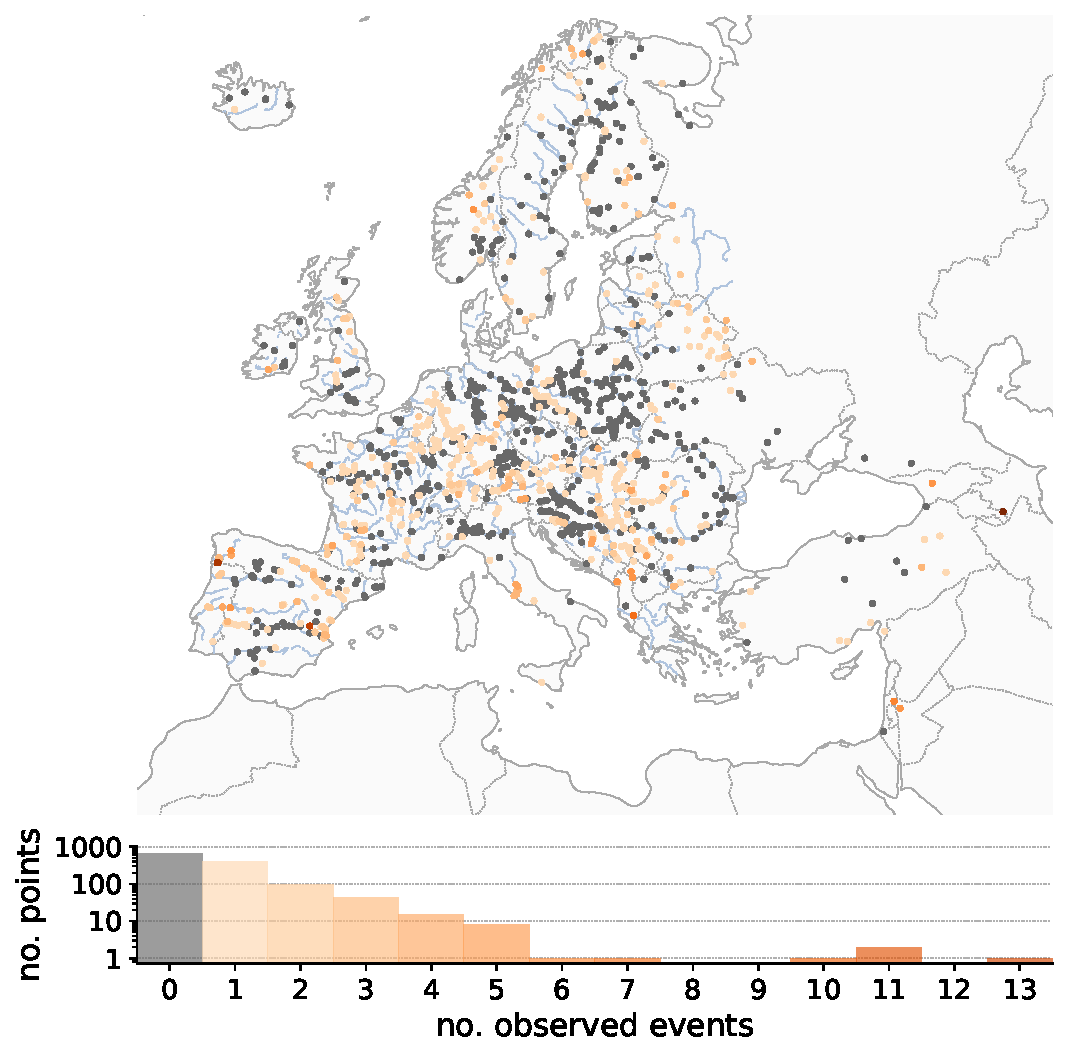
\includegraphics[width=0.5\textwidth]{figureA1.pdf}
    \caption{Geographical distribution of the stations used for optimizing the warning criteria, and number of "observed" flood events during the study period.}
    \label{fig:map_observed}
\end{figure}

The optimization of the warning criteria is based on 1239 stations and 874 "observed events". Throughout the study period, 61\% of the stations did not exceed the 5-year return period, which means that hits and misses cannot exist, and the only term in the contingency table will be false alarms. Consequently, the f-score for these stations can be either 0 or null.

The imposition of a minimum contributing area of 2000 km² places a constraint on the number of stations available for optimization, consequently affecting the count of observed events. In the final phase of our analysis, we assessed the implications of this criterion by expanding our consideration to stations with a minimum area of 500 km². Figure \ref{fig:observed_vs_area} represents the relationship between an increasing catchment area threshold and the corresponding number of stations and "observed" events. By excluding the points with contributing area smaller than 2000 km², we discarded 37\% of the stations and 48\% of the events. The objective of this decision was to use the current warning criteria as benchmark.

\begin{figure}[ht]
    \centering
    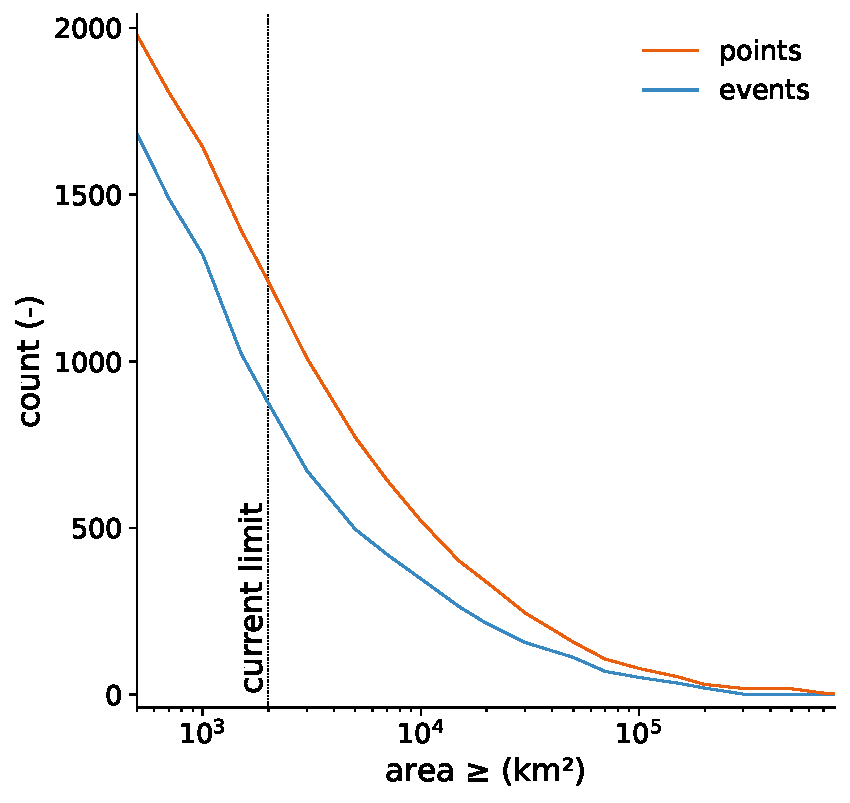
\includegraphics[width=0.425\textwidth]{figureA2.pdf}
    \caption{Number of stations (orange) and observed events (blue) by catchment area threshold. The vertical, dotted line represents a catchment area of 2000 km², the current limit in the EFAS warnings.}
    \label{fig:observed_vs_area}
\end{figure}

\appendix[B]
\appendixtitle{Probabilistic skill of individual NWPs}
\label{appendix:NWP_prob_skill}

In the initial assessment of NWP skill, we calculated the Brier score for each NWP at daily lead times. The Brier score, as an error metric, yields values that can be challenging to interpret, given the dependence of error magnitude on the specific variable —particularly in the context of rare events like floods, where the magnitude is inherently low. Instead, we employ the Brier skill score (BSS) to gauge the relative skill of a model in comparison to a reference. Models outperforming the reference receive a positive BSS, while those underperforming register a negative BSS. For the reference, we opted for a dummy model that never predicts an event ($P_{pred}=0$) \citep{Legg2004}.

\begin{figure}[ht]
    \centering
    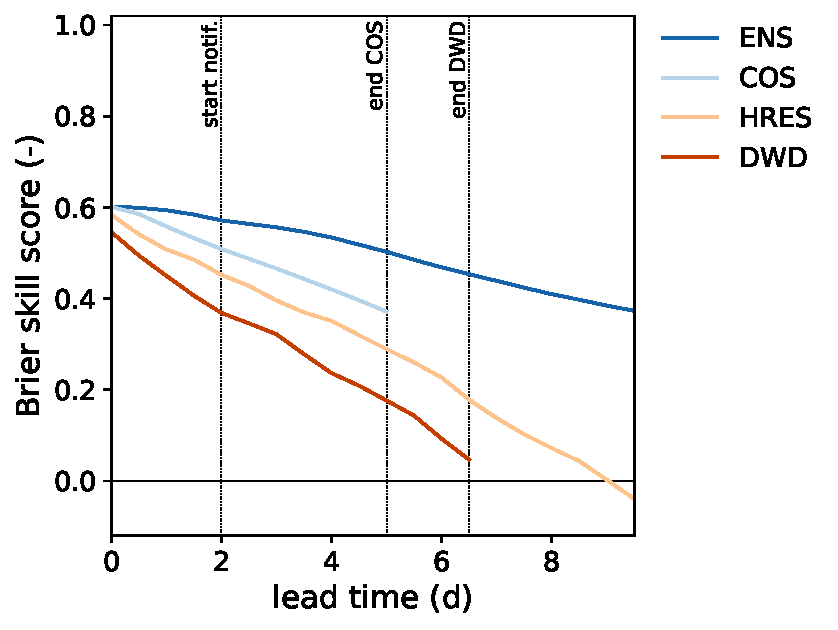
\includegraphics[width=0.45\textwidth]{figureB1.pdf}
    \caption{Brier skill score of the four NWP used in EFAS at daily lead times. The reference ($BSS=0$) is a model that never predicts an event. Blue lines represent probabilistic models, and orange lines deterministic ones.}
    \label{fig:BSS}
\end{figure}

The plot above demonstrates that probabilistic models exhibit greater skill than deterministic ones. Only within very short lead times (0-1 days) do deterministic models approximate the skill of probabilistic models. This is particularly significant for EFAS warnings, as warnings are issued only at lead times longer than 2 days (indicated by  the leftmost dotted line). As lead time increases, there is a degradation in skill. This decline impacts ENS to a lesser extent than the other models. Both deterministic models display poor skill at their forecast horizon.

\appendix[C]
\appendixtitle{Roebber diagram: a visual summary of the results}
\label{appendix:roebber}

The Roebber diagram in Figure \ref{fig:roebber} offers an alternative perspective on the results of the optimization of the warning criteria. Roebber diagrams condense four skill metrics into a single plot, with an ideal model positioned at the top right corner \citep{Roebber2009}. The figure \ref{fig:roebber} shows simultaneously the skill of the current warning criteria, the optimization of individual NWP (Table \ref{tab:NWP_optimization}), and the optimization of combination methods (Table \ref{tab:COMB_optimization}) for the lead time range 2-5.5 days.

\begin{figure}
    \centering
    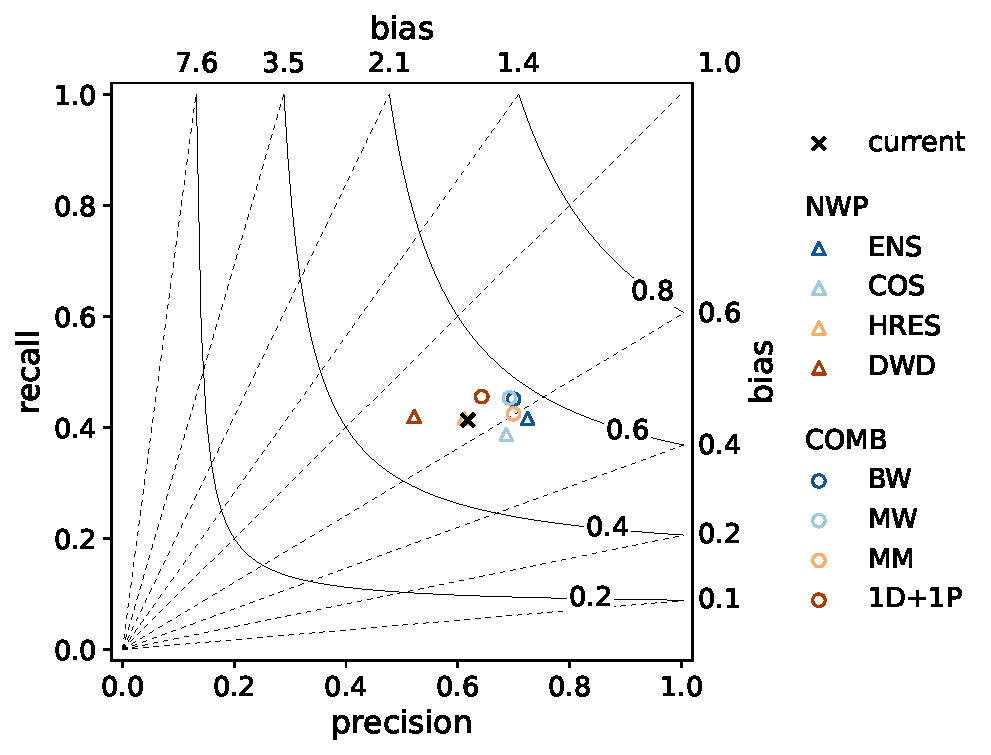
\includegraphics[width=0.475\textwidth]{figureC1.pdf}
    \caption{Roebber diagram of the optimized criteria at the lead time range from 2 to 5.5 days. Four skill metrics are represented: precision and recall in the X and Y axis, bias by the dashed lines, and the $f_{0.8}$ score by the solid lines. Triangles illustrate individual NWP and circles the combination of NWP. For reference, the skill of the current warning criteria is shown as a black cross.}
    \label{fig:roebber}
\end{figure}

All NWP models and the current criteria exhibit negative bias, indicating that EFAS underpredicts the occurrence of flood events. In the case of the optimizations carried out in this analysis, the selection of the $f_{0.8}$ score as the target metric in the optimization forces this bias, as it prioritizes precision over recall. It is remarkable that the improved $f_{0.8}$ of the probabilistic models is a result of higher precision, while recall values remain similar across all NWPs and the current criteria.



%%%%%%%%%%%%%%%%%%%%%%%%%%%%%%%%%%%%%%%%%%%%%%%%%%%%%%%%%%%%%%%%%%%%%
% REFERENCES
%%%%%%%%%%%%%%%%%%%%%%%%%%%%%%%%%%%%%%%%%%%%%%%%%%%%%%%%%%%%%%%%%%%%%

\bibliographystyle{ametsocV6}
\bibliography{references}


\end{document}